\documentclass[dutch]{book}
\usepackage{amsmath}
\usepackage{hyperref}
\usepackage{listings}
\usepackage{graphicx}
\usepackage{enumitem}
\usepackage{siunitx}
\usepackage{float}
\usepackage{babel}

\lstset
{ %Formatting for code in appendix
	language=Python,
	basicstyle=\footnotesize,
	numbers=left,
	stepnumber=1,
	showstringspaces=false,
	tabsize=1,
	breaklines=true,
	breakatwhitespace=false,
	frame=single,
}

% \begin{reusefigure}[<float spec>]{<ref>}
\newenvironment{reusefigure}[2][htbp]
{\addtocounter{figure}{-1}%
	\renewcommand{\theHfigure}{dupe-fig}% If you're using hyperref
	\renewcommand{\thefigure}{\ref{#2}}% Figure counter is \ref
	\renewcommand{\addcontentsline}[3]{}% Avoid placing figure in LoF
	\begin{figure}[#1]}
	{\end{figure}}

% Title Page
\title{Python Cookbook voor MTE}
\author{W.M. Jutte en J. Antonissen}


\begin{document}
	
	\frontmatter
	\maketitle
	%\input{Glossaries}
	%\input{Preface}
	%\input{Abstract}
	\tableofcontents
	
	\mainmatter
	\part{CircuitPython}
	\chapter{Getting Started}

\section{Introduction}
	De CircuitPython omgeving is ontworpen voor beginners in software en elektronica. Voordat je met het CircuitPython bordje aan de slag kan moet het \'e\'en en ander worden ge\"installeerd en ge\"updatet. Adafruit heeft een beginners tutorial voor CircuitPython die je gaat doorlopen in ~\ref{sec:CircuitPythonTutorial}.%, maar de Adafruit Metro M4 Express heeft een WIFI module die eerst ge\"updatet moet worden.

%\section{Updaten van de WIFI module}
	
	%Als je Windows 7 gebruikt moet je eerst de nieuwste drivers installeren van de volgende link:\\
	%\url{https://github.com/adafruit/Adafruit_Windows_Drivers/releases}\\
	%Mac en Linux gebruikers hoeven geen drivers te installeren.\\
	
%Als je al eens code op de CIRCUITPY drive hebt gezet, maak dan een back-up, want het wordt overschreven door de code die je nu gaat uploaden. Als dit de eerste keer is dat je het bordje gebruikt kan je de back-up overslaan.\\
	
	%\noindent Download de  Metro\_M4\_WIFI\_ESP32\_Passthru.uf2 file van:\\
	%\url{https://learn.adafruit.com/upgrading-esp32-firmware/upgrade-an-airlift-all-in-one-board}\\
	
	
	%\noindent Zoek het reset knopje op je bordje. Het is een klein zwart knopje, te zien in figuur \ref{fig:ResetButton}. Druk twee keer op dit knopje om het bordje in de bootloader te zetten. Als het niet de eerste keer lukt, probeer het dan opnieuw. Het ritme moet goed zijn en dat kan een paar pogingen kosten. Als het is gelukt zal de RGB LED op het bordje rood knipperen en daarna groen blijven. Een nieuwe schijf genaamd bordnaamBOOT zal verschijnen als in figuur \ref{fig:Bootloader}, waar bordnaam een referentie naar de naam van je bord is.\\
	
%	\begin{figure}[!htb]
%		\center{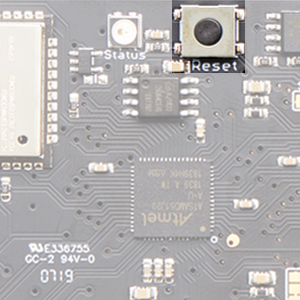
\includegraphics[width=0.3\linewidth]{figures/ResetButton.png}}
%		\caption{De reset knop}
%		\label{fig:ResetButton}
%	\end{figure}
	
	
%	\begin{figure}[!htb]
%		\center{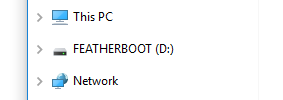
\includegraphics[width=0.6\linewidth]{figures/Drive.png}}
%		\caption{De micro-controller in bootloader}
%		\label{fig:Bootloader}
%	\end{figure}
	
%	\newpage\noindent Het bordje is nu in bootloader mode. Zoek de UF2 file die je net hebt gedownload en sleep het naar de BOOT schijf op je computer zoals in figuur \ref{fig:UF2}. De lichtjes knipperen nu opnieuw en de BOOT schijf verdwijnt.\\

%\footnotesize\noindent Originele bron: \url{https://learn.adafruit.com/upgrading-esp32-firmware/upgrade-an-airlift-all-in-one-board}
%\normalsize

%\begin{figure}[H]
%	\center{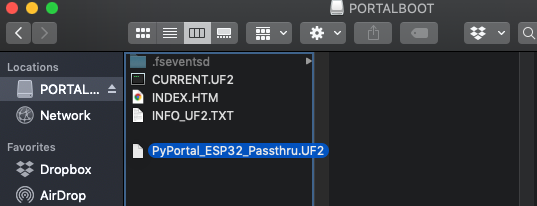
\includegraphics[width=\linewidth]{figures/UF2_install.png}}
%	\caption{Sleep de UF2 file naar de BOOT drive}
%	\label{fig:UF2}
%\end{figure}

\section{Welcome to CircuitPython tutorial}\label{sec:CircuitPythonTutorial}
	Alle andere benodigdheden om te starten met CircuitPython wordt behandelt in Adafruit's kennismaking tutorial. Doorloop Adafruits' \textbf{"Welcome to CircuitPython"} tutorial tot en met het kopje \textbf{"CircuitPython Libraries"} op:\\
	
	\url{https://learn.adafruit.com/welcome-to-circuitpython/} \\

Op deze website staat de basis van cirquit python, lees dit goed door. Download ook \href{https://codewith.mu/}{de Mu editor} zoals op de guide staat aangegeven. \\
	
	\url{https://codewith.mu/}


\section{Plotten met Mu editor}\label{sec:plotter}
In de Mu editor zit een ingebouwde plotter. Dit is erg handig om bijvoorbeeld sensordata direct te plotten. Om gebruik te maken van de plotter moet data in een tuple geprint worden. Open mu editor om dit te testen. Klik op Serial en Plotter bovenaan mu editor. Als het goed is ziet je scherm eruit als figuur~\ref{fig:SerialPlotter}. Als er een programma loopt, klik dan in het vak van de repl en doe ctrl+c om de code te stoppen en druk op een een willekeurige knop om in de repl te gaan. Print nu een paar tuples. Een tuple is een datastructuur dat normale haakjes () gebruikt. Type in de repl bijvoorbeeld de volgende commands, print((1,2)), print((3,2)), a=(0,0), print(a). Als het goed is zie je dan hetzelfde als in figuur~\ref{fig:TuplePlot}. Probeer ook \'e\'en getal te plotten door bijvoorbeeld print((4)) te typen. Als het goed is zie je niks gebeuren. Dit komt door een eigenaardigheid in python dat een enkel getal in een tuple geschreven moet worden als (4,) en niet (4) . Als je print((4,)) typt wordt de waarde wel geplot.

\begin{figure}[H]
	\center{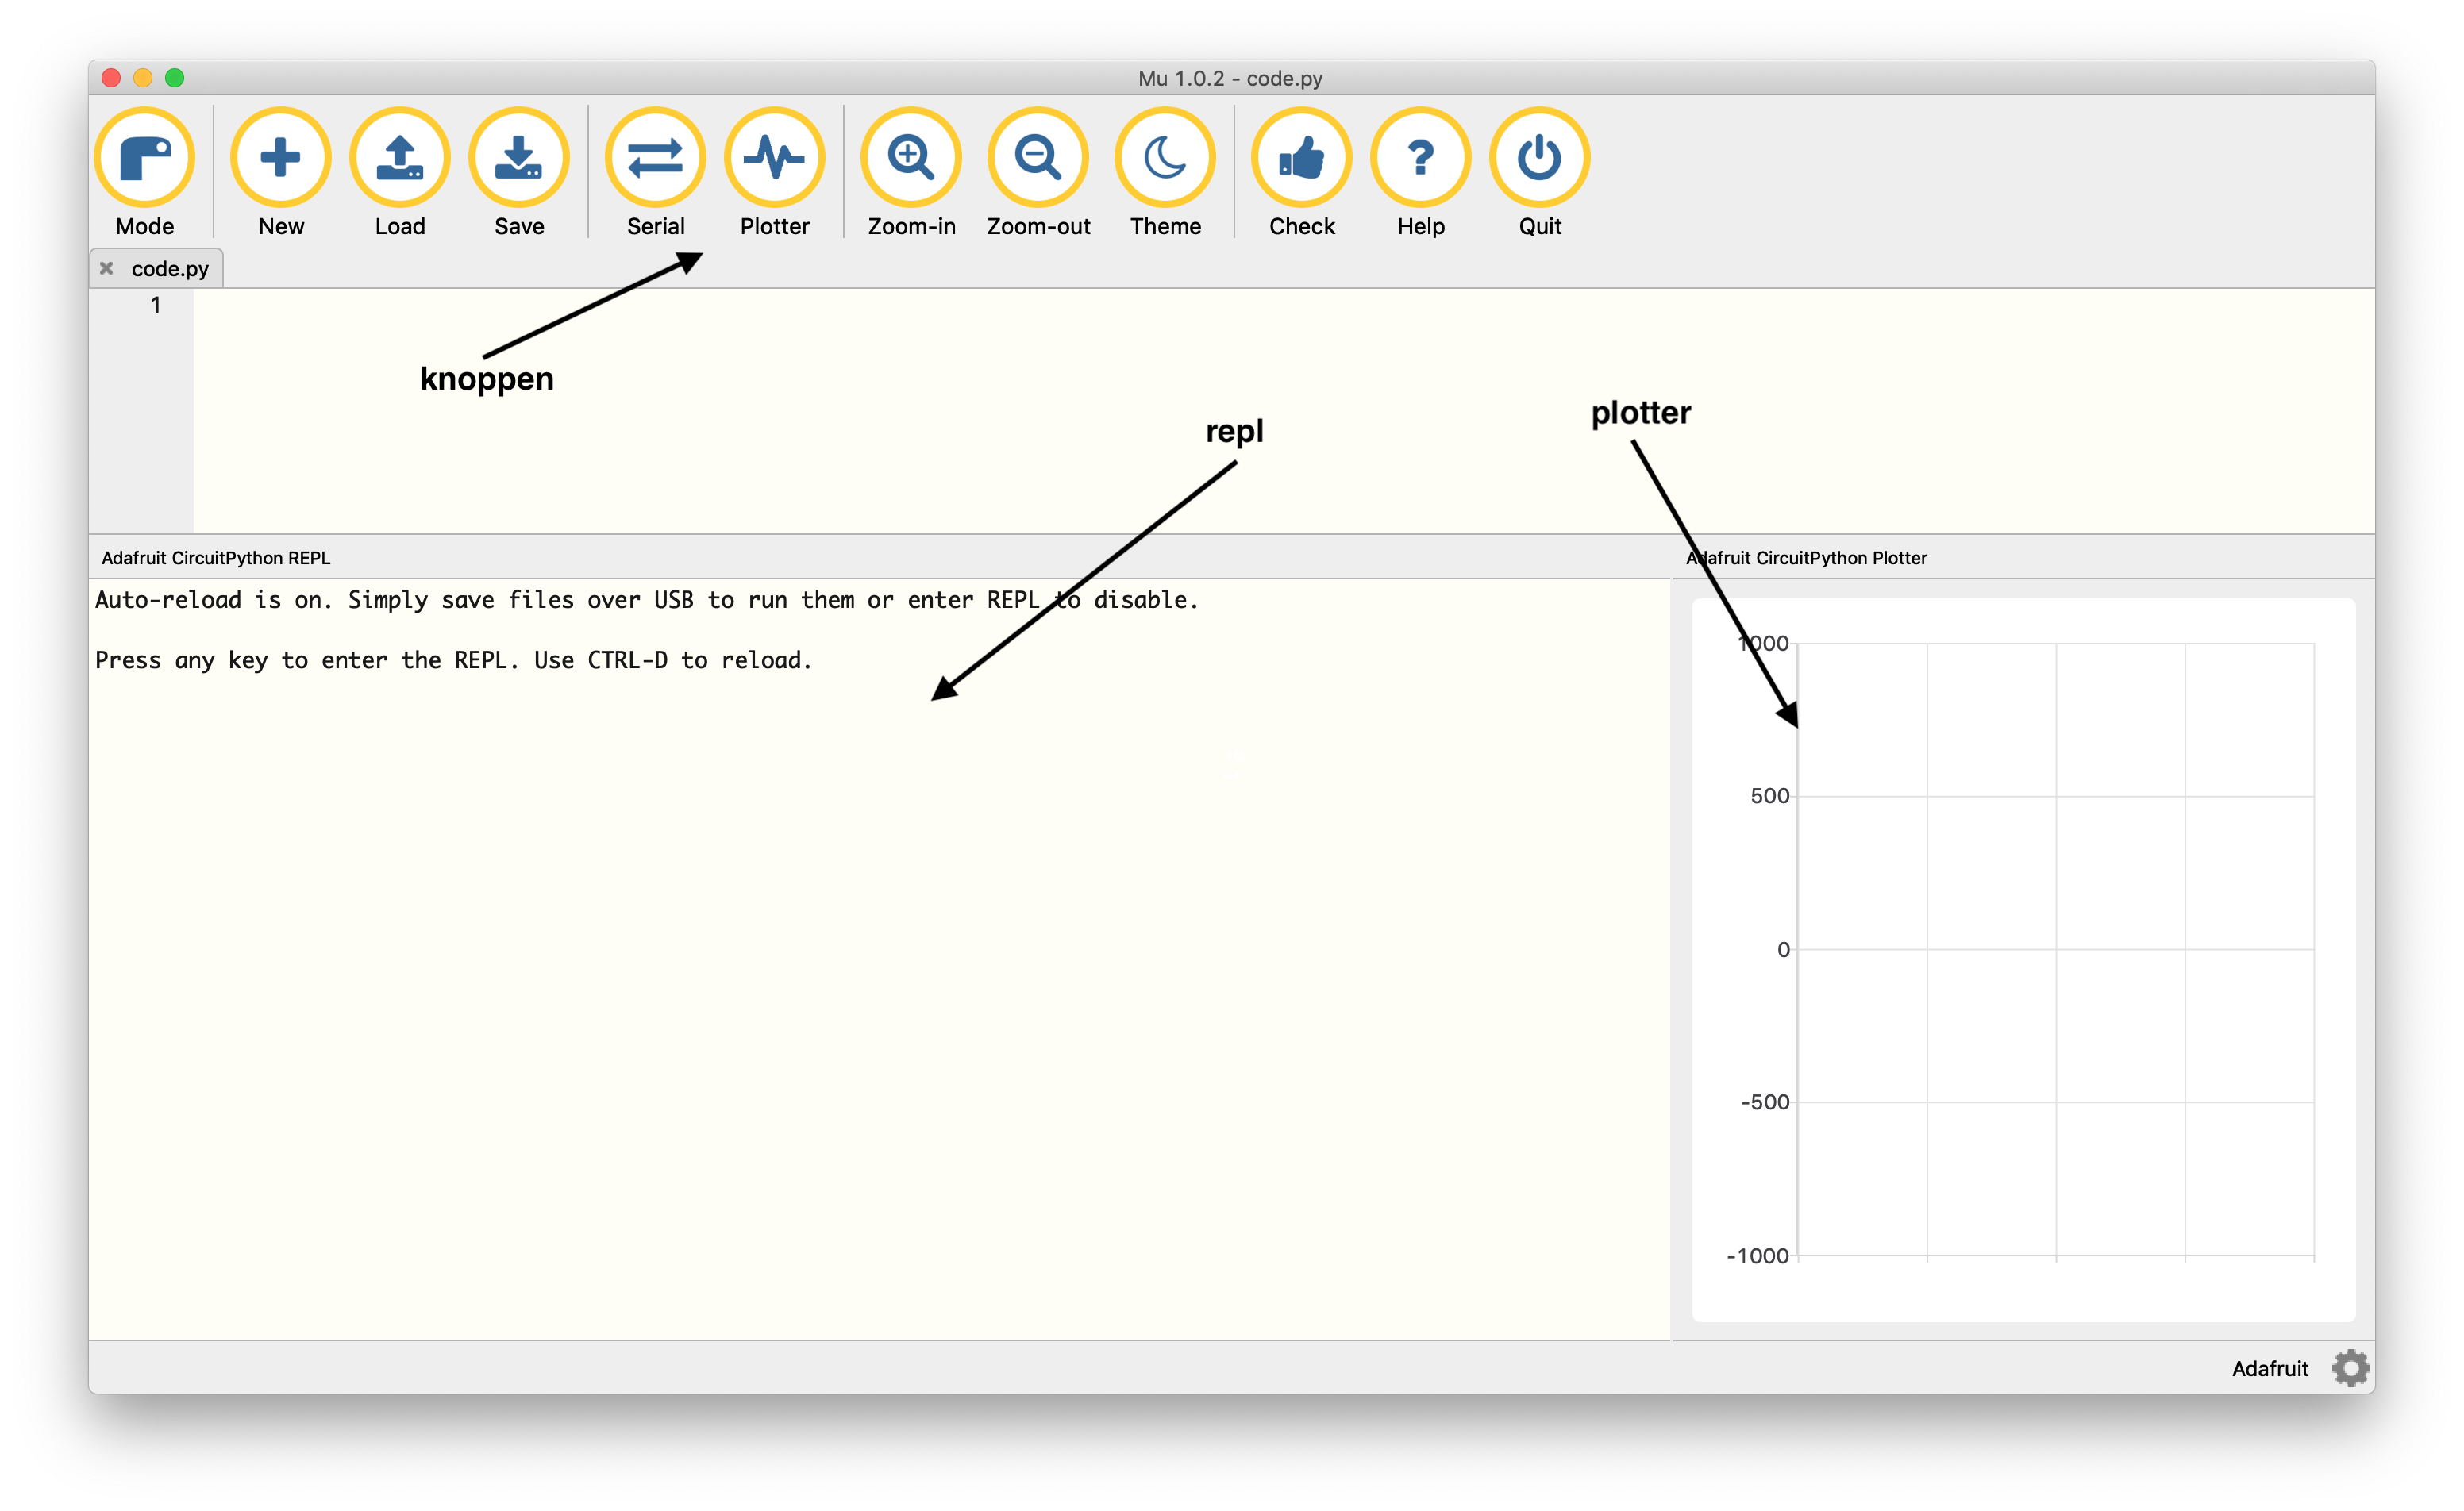
\includegraphics[width=0.9\linewidth]{figures/SerialPlotter.png}}
	\caption{Mu editor met de REPL en plotter open}
	\label{fig:SerialPlotter}
\end{figure}

\begin{figure}[H]
	\center{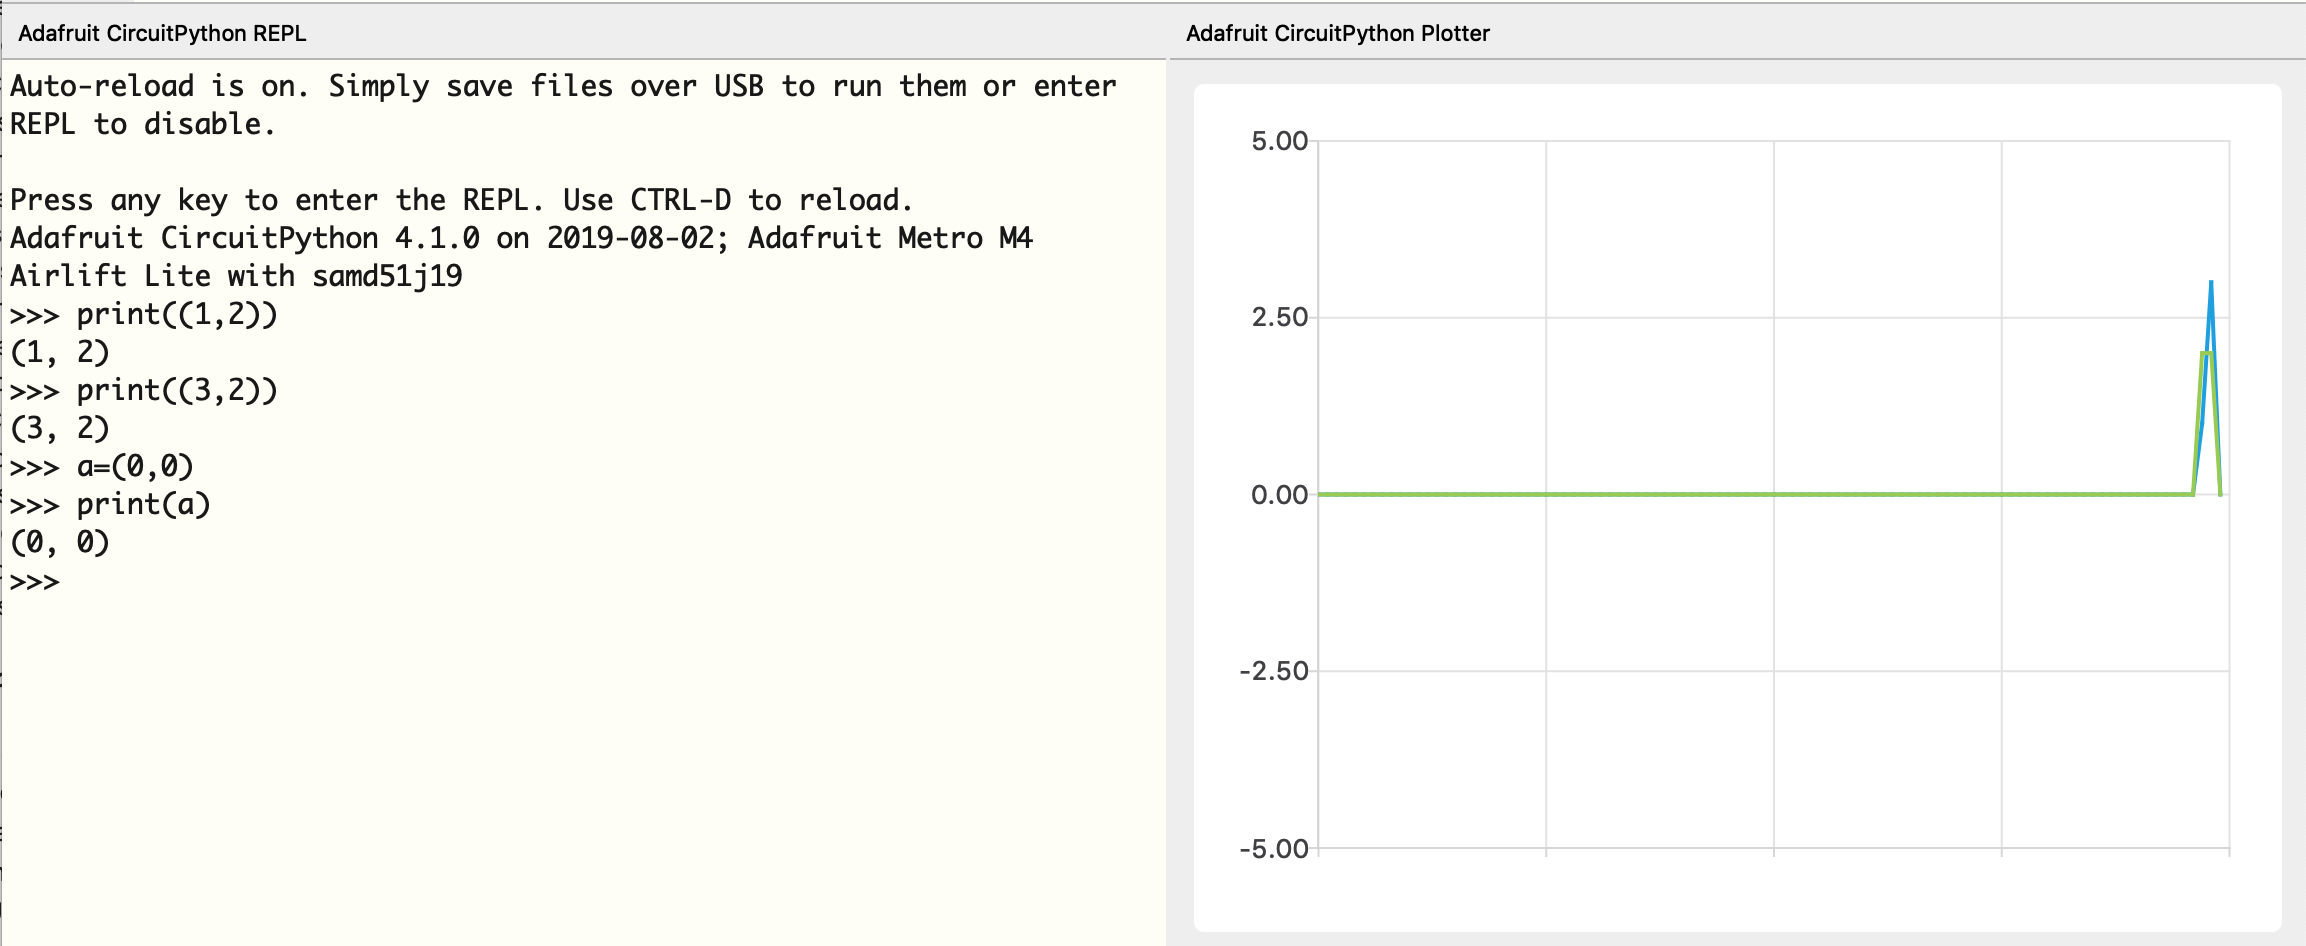
\includegraphics[width=0.9\linewidth]{figures/TuplePlot.png}}
	\caption{Plotten van tuples}
	\label{fig:TuplePlot}
\end{figure}


\url{https://learn.adafruit.com/make-it-graph-plot}

\newpage
\section{Een extra woord over bibliotheken}\label{sec:library}
In deze handleiding wordt gebruik gemaakt van de volgende bibliotheken:
\begin{itemize}
	\item adafruit\_bus\_device map
	\item adafruit\_esp32spi map
	\item adafruit\_hcsr04.mpy
	\item adafruit\_motor map
	\item neopixel.mpy
\end{itemize}

Haal de up-to-date bibliotheken uit adafruits library bundle en zet ze in de lib folder van je CIRCUITPY drive. De bundel is te downloaden op \\

\url{https://circuitpython.org/libraries}. \\

Let op, je kan niet alle bibliotheken op het bordje zetten, hiervoor is niet genoeg ruimte. Zet dus alleen de bibliotheken die je gebruikt op het bordje.


\section{Veilig omgaan met het bordje}\label{sec:VeiligOmgaan}
De bordjes kunnen kapot gaan als de pinnen op het bordje teveel stroom moeten leveren of als er teveel stroom het bordje instroomt. Het Adafruit Metro M4 Express bordje heeft een \SI{3.3}{\volt}, \SI{5}{\volt} en een $V_{in}$ output pin, te zien in figuur~\ref{fig:MetroM4}. Deze pinnen kunnen bij elkaar maximaal \SI{500}{\milli\ampere} leveren en kunnen gebruikt worden om je projectje te voorzien van stroom. Alle andere pinnen op het bordje zijn I/O pinnen en zijn niet bedoeld om zulke hoge stroom te leveren. In de datasheet van de ATSAM51D wordt een maximum van \SI{2}{\milli\ampere} per I/O pin aangegeven. Als je je hier niet aan houdt is het mogelijk dat componenten in het bordje doorbranden. Zie \url{https://www.alanzucconi.com/2016/09/17/how-to-destroy-an-arduino-board/} voor meer informatie over hoe je een bordje kapot kan maken.

\begin{figure}[!htb]
	\center{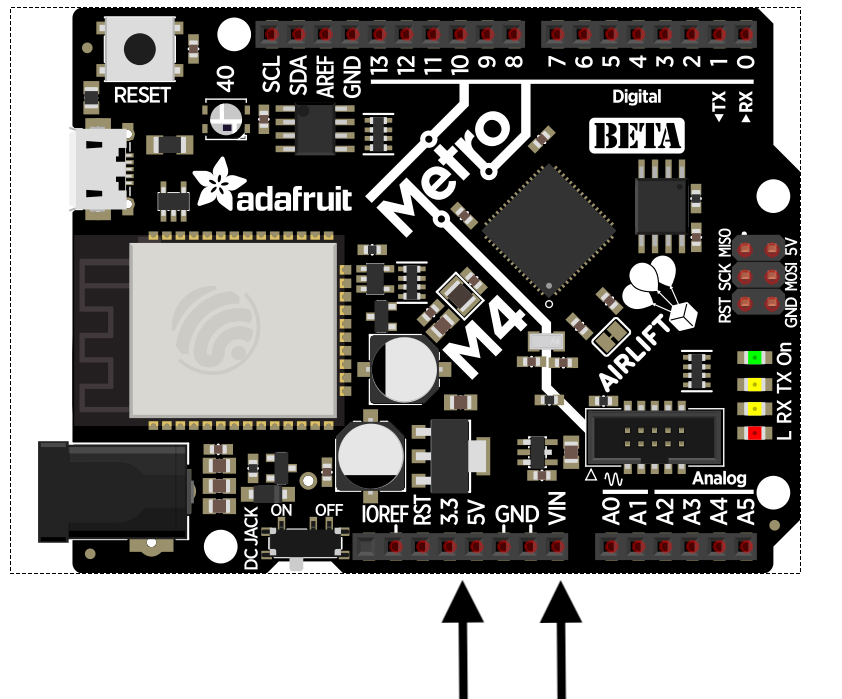
\includegraphics[width=0.8\linewidth]{figures/MetroM4.png}}
	\caption{De spanningsbronnen op de Metro M4 Express}
	\label{fig:MetroM4}
\end{figure}

\clearpage
\newpage

\section{Bordje updaten}

\begin{center}
    Let op: dit alleen uitvoeren als de docent hier om vraagt!
\end{center}

Het bordje kan ge\"{u}pdatet worden door het bordje in de bootloader modus te zetten en het update bestand erop te slepen. \\

Download eerst de update van de bootloader op de volgende link (onderaan op pagina). Let op download alleen se stabiele versie, dus geen alpha of beta builds. \\

\url{https://circuitpython.org/board/metro_m4_airlift_lite/} \\

Klik twee keer op reset om Het bordje in bootloader modus te zetten. Sleep vervolgens het update bestand (de nieuwe bootloader) op het bordje. Het bordje zal opnieuw opstarten. Na het updaten van de bootloader zal CirquitPython van het bordje zijn verdwenen, deze moet er dus opnieuw worden opgezet. Download op dezelfde pagina ook de laatste versie van CirquitPython, zet het bordje weer in bootloader modus en sleep het cirquitPython bestand naar de bootloader. Het bordje zal weer opnieuw opstarten. \\

Gefeliciteerd, je hebt nu de bootloader en CirquitPython ge\"{u}pdatet!


	\chapter{Frequently Asked Questions}

\section{Bordje problemen}

Het aansluiten van het bordje kan soms lastig zijn. Hieronder een aantal tips: \\

\noindent \textbf{USB kabel} \\

Voor het aansluiten van het bordje heb je een USB-A naar micro-USB kabel nodig. Sommige van deze kabels zullen niet werken, deze leveren bijvoorbeeld wel stroom naar geen date. Als het bordje niet werkt,bijvoorbeeld als hij wel aan gaat maar windows geen verbinding kan maken, probeer dan dus eerst altijd een andere kabel. Pas na 3 kabeltjes kan je met enige zekerheid zeggen dat je dit probleem hebt verholpen. \\

\noindent \textbf{Anti virus} \\

Sommige anti-virus software blokkeren USB apparaten. Probeer dus ook eens je bordje aan te sluiten terwijl je anti-virus programma uit staat.\\

\noindent \textbf{Bordje niet gevonden} \\

Het kan zijn dat de verkeerde bootloader op het bordje staat. Volg de stappen in het hoofdstuk bordje updaten om de bootloader te updaten en CirquitPython op het bordje te zetten. \\

\url{https://circuitpython.org/board/metro_m4_airlift_lite/}

\clearpage
\newpage

\section{Code Problemen}

Bij het coderen kunnen veel fouten krijgen. Een computer (en dus ook het bordje) werkt alleen als de code erop foutloos is. \\

Let bij het schrijven van het programma op het volgende: \\

\noindent \textbf{Serial en Code check} \\

In MU zitten de 'Serial (of REPL)' en 'Code Check' knoppen. Hiermee kan je goed  controleren of er fouten in je code zitten. De Serial knop geeft in een schermpje onderaan aan welke fouten er in je code zitten, hierbij staat ook op welke regel zich de fout bevind. De Code Check knop controleert de code tussen de code door. \\

\begin{figure}[h!]
    \centering
    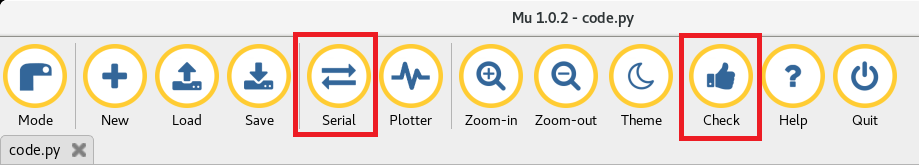
\includegraphics{figures/check.png}
    \caption{Serial en Code Check}
    \label{fig:my_label}
\end{figure}

\noindent \textbf{Code problemen} \\

\noindent Kom je er niet uit ? check dan het volgende lijstje: \\

\begin{itemize}
    \item Heet het bestand op het bordje code.py ?
    \item Staat jou code.py bestand op het bordje ?
    \item Staat jou code in het bestand code.py ?
    \item Zitten er typ fouten in je code ?
    \item Staan er onnodige spaties of hoofdletters in je code ?
    \item Stuur je de poorten aan die je wilt gebruiken ?
\end{itemize}
	\chapter{Ledjes}\label{chap:ledjes}
In de introductie heb je kennis gemaakt met CircuitPython en Mu editor en heb je een ledje op het bordje zelf aangestuurd. Een micro-controller wordt voornamelijk gebruikt om externe hardware aan te sturen. In dit hoofdstuk worden ledjes op verschillende manieren aangestuurd. Een ledje laten branden is niet heel spannend, maar het is \'e\'en van de simpelste manieren om code te testen. Het maken van een led circuit is erg eenvoudig en je krijgt gelijk visuele feedback. Ook zit tussen het aansturen van een ledje of een motor weinig verschil.

\newpage
\section{Extern LEDje laten branden}\label{sec:ledExtern}
	\paragraph{Probleem:} Je wilt een externe LED laten knipperen.
	\paragraph{Benodigdheden:}
	\begin{itemize}
		\item 1x LED
		\item 1x \SI{680}{\ohm} weerstand (Of weerstand die in de buurt komt)
	\end{itemize}
	\paragraph{Oplossing:}
		\begin{figure}[H]
			\center{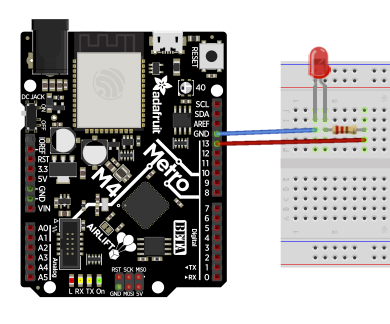
\includegraphics[width=0.6\linewidth]{figures/LED.png}}
			\caption{Led Circuit}
			\label{fig:LED}
		\end{figure}
		\lstinputlisting{code/LED.py}

	\paragraph{Discussie:}  Om een ledje te laten knipperen zijn drie modules nodig. De "board" module, zodat de pinnen aangeroepen kunnen worden met het nummer dat op het bordje staat. De "time" module om gebruik te kunnen maken van tijd en timing functies en de digitalio module zodat de I/O pinnen ingesteld kunnen worden. \\
	
	De LED zit aangesloten op pin 13 en kan daarom aan en uit gezet worden door de spanning op pin 13 hoog en laag te zetten. In de code kan je controle krijgen over pin 13 met het gebruik van de DigitalInOut() functie van de digitalio module. De functie neemt als parameter het nummer van de pin dat je wilt gebruiken en cre\"eert dan een 'object', zodat je pin 13 met code kan aansturen. In de code krijgt het object de naam led toegewezen. Een I/O pin kan zowel voor het uitlezen en het aansturen van spanning gebruikt worden. In de code moet daarom verteld worden hoe we de pin willen gebruiken. Om de I/O pin voor aansturen te gebruiken wordt de "direction" eigenschap van het led object op output gezet.\\
	
	Na het initialiseren van de pin kan de spanning hoog en laag gezet worden door de "value" eigenschap van het led object respectievelijk de waarde True of False te geven. De time.sleep() functie wordt gebruikt om de code te vertragen tussen het aan en uit zetten.
	
\newpage
\section{Meerdere LEDjes}\label{sec:meerdereLedjes}
	\paragraph{Probleem:} Je wilt meerdere ledjes tegelijkertijd en onafhankelijk van elkaar aansturen.
	\paragraph{Benodigdheden:}
		\begin{itemize}
			\item 8x LED
			\item 8x \SI{680}{\ohm} weerstand
		\end{itemize}
	\paragraph{Oplossing}:
	\begin{figure}[H]
		\center{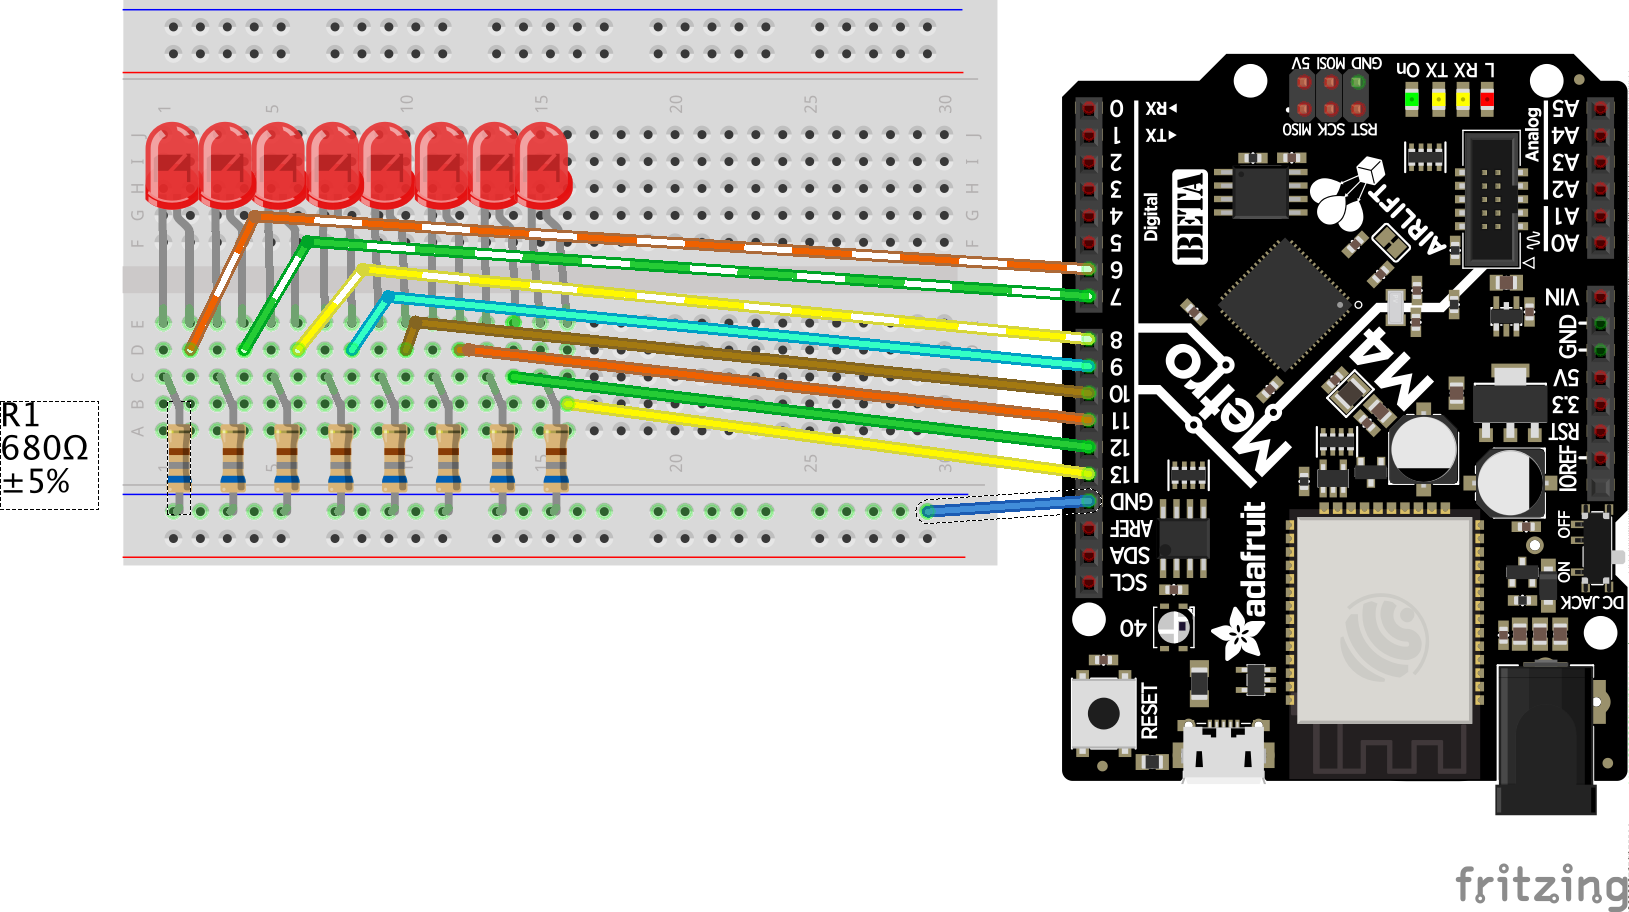
\includegraphics[width=\linewidth]{figures/MultipleLED.png}}
		\caption{Acht Ledjes}
		\label{fig:MultipleLED}
	\end{figure}
\newpage
	\lstinputlisting{code/Multiple_LED.py}
	\paragraph{Discussie:} Voor elk ledje moet 1 pin ge\"initialiseerd worden. Voor 8 ledjes moeten dus 8 pinnen op digitale output gezet worden. Dit gaat hetzelfde als met 1 ledje als in recept~\ref{sec:ledExtern}. Daarna worden alle ledjes in een lijst gezet, zodat met een for loop door de ledjes gelooped kan worden. In de oneindige while loop gaat het programma gelijk de eerste for loop in. Hier worden de ledjes \'e\'en voor \'e\'en aangezet in de volgorde van ledlist met \SI{0.2}{\second} wachtijd tussen elk ledje. Vervolgens gaat het de tweede for loop in, waar de ledjes in omgekeerde volgorde van de ledlist worden uitgezet. 

\newpage
\section{Meerdere LEDjes met minder pinnen door middel van een shiftregister}
	\paragraph{Probleem:} Je wilt meerdere ledjes aansturen, maar wilt niet per ledje 1 pin opofferen.
	\paragraph{Benodigdheden:}
		\begin{itemize}
			\item 8x LED
			\item 8x \SI{680}{\ohm} weerstand (in dit geval mag een lagere weerstand van \SI{220}{\ohm} gebruikt worden omdat de stroom niet door de I/O pinnen wordt geleverd)
			\item 1x SN74HC595N shift register
		\end{itemize}
	\paragraph{Oplossing}:
	\begin{figure}[H]
		\center{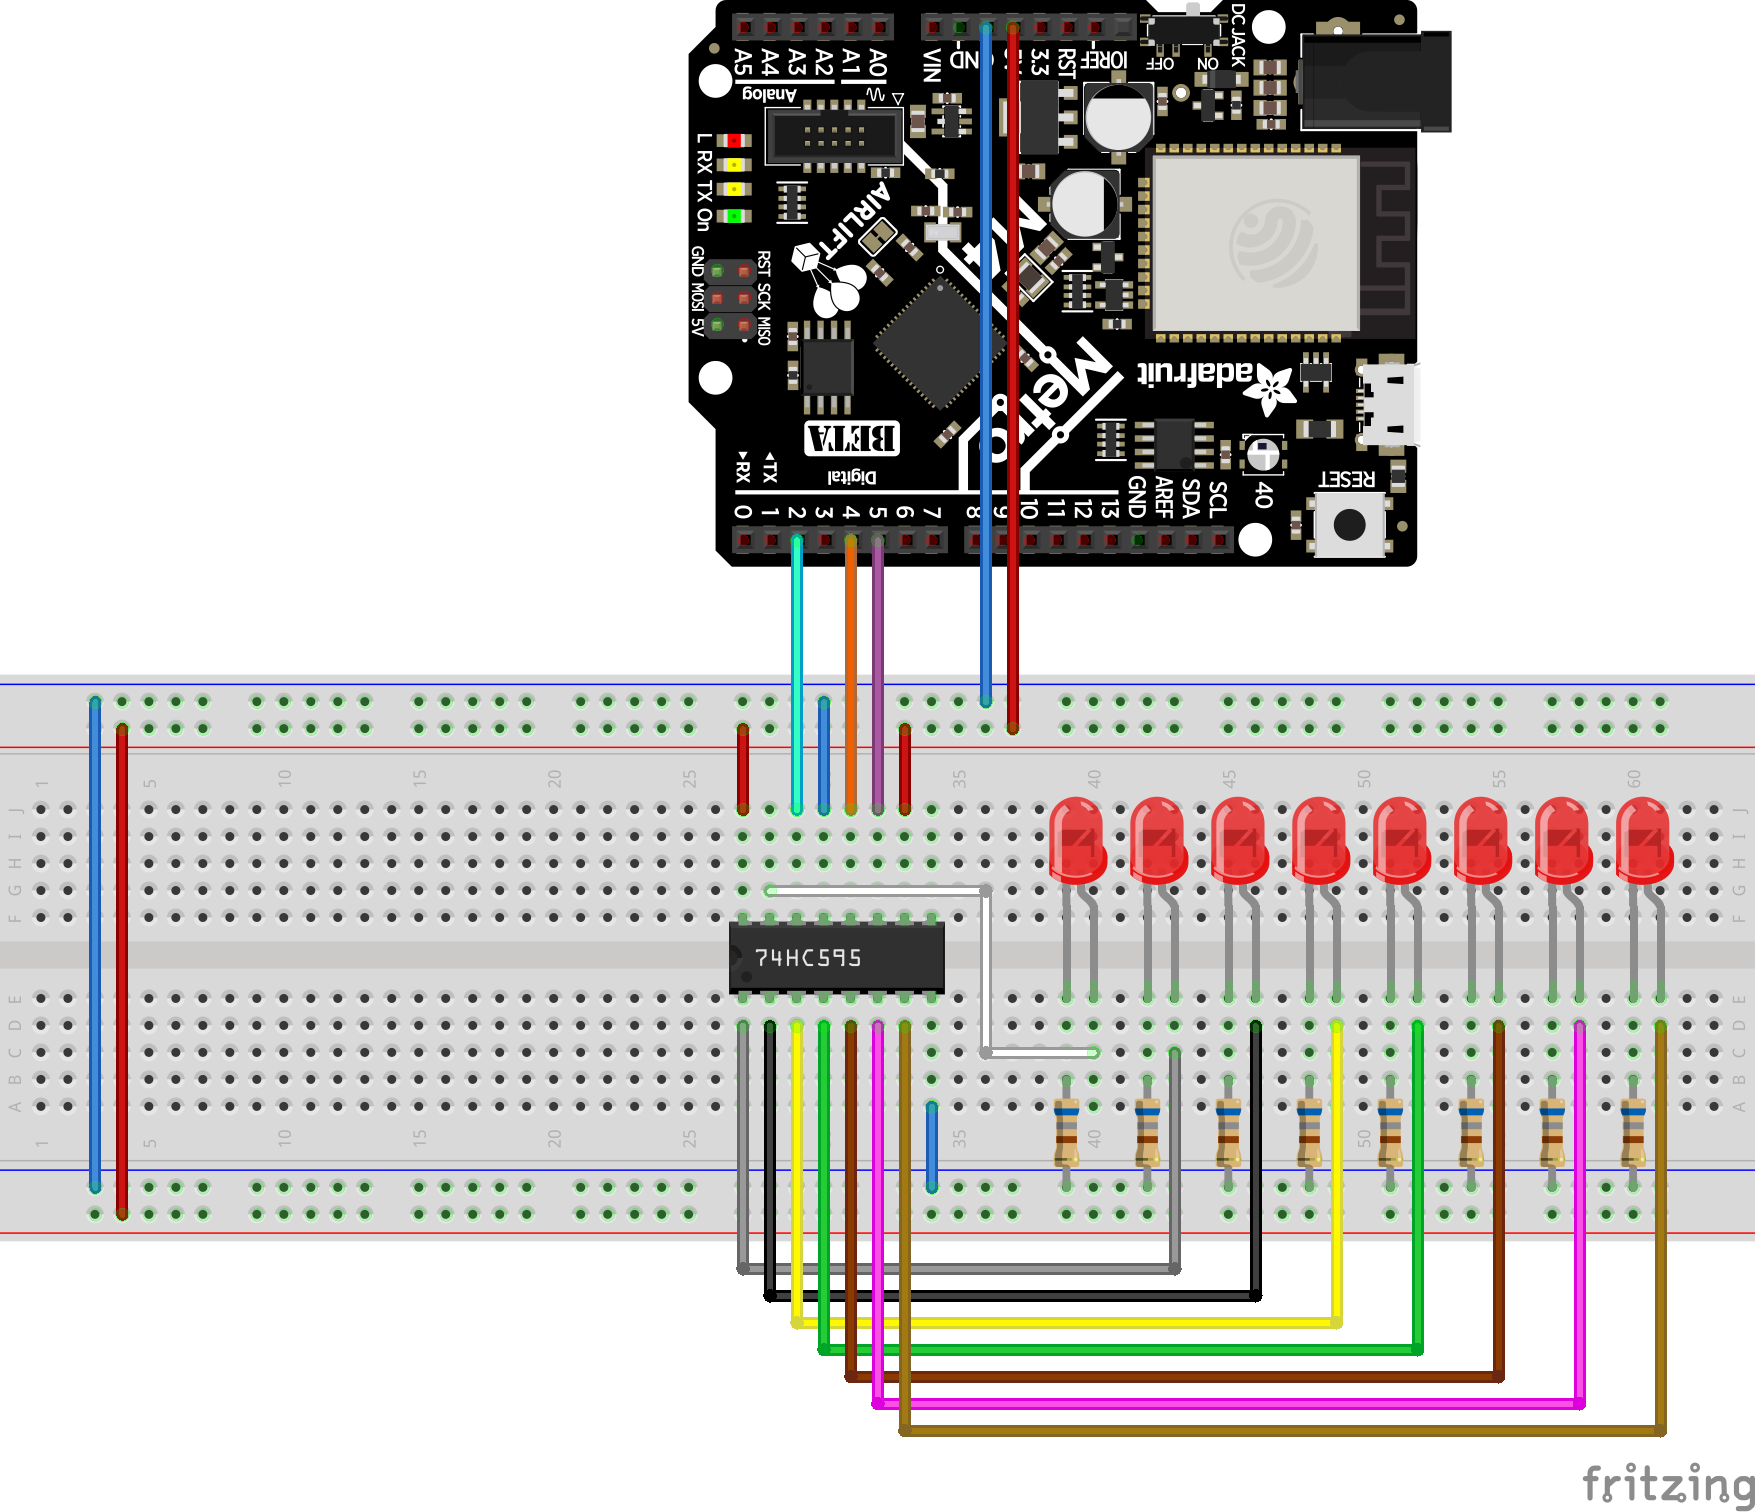
\includegraphics[width=0.75\linewidth]{figures/ShiftRegister.png}}
		\caption{Acht ledjes met een shiftregister}
		\label{fig:ShiftRegister}
	\end{figure}
	
	\clearpage
	\newpage
	
	\lstinputlisting{code/Shiftregister.py}
	\newpage
	\paragraph{Discussie:} Een shiftregister wordt gebruikt om een groot aantal ledjes (of iets anders) aan te sturen, zonder dat je voor elk ledje een nieuwe pin nodig hebt, zoals in recept~\ref{sec:meerdereLedjes}. Je kunt met 3 I/O pinnen een oneindig aantal ledjes aansturen als je meerdere shiftregisters aan elkaar koppelt. Het gebruik van een shiftregister is wel iets complexer. Dus hoe werkt het?
	
	Het schema van het shiftregister is te zien in figuur~\ref{fig:SN74HC595N}. 
	\begin{enumerate}
		\item Qa, Qb.... ,Qh zijn de pinnen waar de ledjes op aangesloten worden.
		\item Vcc en GND zijn de pinnen die de stroom aan zowel de ledjes als de IC leveren.
		\item De $\overline{OE}$ pin schakelt Qa-Qh tegelijk uit als er een hoge spanning op staat. In ons geval is het niet nodig om Qa-Qh tegelijk uit te zetten, dus kan de pin direct op ground aangesloten worden.
		\item De $\overline{SRCLR}$ pin cleared het shift register als er een lage spanning op gezet wordt. Dit is onnodig, dus deze pin wordt aangesloten op 3.3V, net als Vcc.
		\item $Q_{H'}$ kun je gebruiken om meerdere IC's aan elkaar te koppelen, dat hier niet wordt gedaan. Deze kan dus open blijven.
	\end{enumerate}  
	
	De overgebleven SER, RCLK en SRCLK worden gebruikt om Qa-Qh in te stellen, waar de ledjes aan vast zitten. Een shiftregister werkt met het principe van doorschuiven. Het shiftregister heeft 8 stukjes geheugen, \'e\'en register per Q pin. Als de SRCLK pin van een lage naar een hoge spanning gebracht wordt, wordt een 1 of een 0 in het register van Qa gezet, afhankelijk van of de spanning op de SER pin respectievelijk hoog of laag is. Tegelijkertijd schuift de waarde die in het register van Qa stond naar Qb, van Qb naar Qc, etc.. Door de gewenste waardes in de goede volgorde op de SER pin te zetten en de SRCLK van laag naar hoog te brengen kunnen de gewenste waarden in de registers van de Q-pinnen gezet worden. Voordat de waarden actief worden moet de RCLK van laag naar hoog gebracht worden.
	
	Het gebruik van het shiftregister werkt als volgt. Eerst zet je RCLK en SRCLK laag. Wat je als eerst op de SER pin zet bepaald uiteindelijk of de laatste pin $Q_H$ aan of uit gaat staan. Als je het ledje op $Q_H$ aan wilt, zet je een hoge spanning op de SER pin en breng je SRCLK van laag naar hoog. In het register van Qa komt nu een 1. Vervolgens breng je SRCLK weer laag en bepaal je of $Q_G$ aan of uit moet. Als Qh uit moet, zet je een lage spanning op de SER pin en breng je SRCLK weer naar hoog. De 1 van Qa schuift door naar Qb en in Qa komt nu een 0. Dit doe je in totaal acht keer tot alle waarden in de registers staan. Tot slot breng je RCLK van laag naar hoog om het definitief te maken en gaan de gewenste ledjes aan de Q-pinnen branden.
	
	Dit proces is gecodeerd in de writereg() functie. Je geeft de functie een lijst met welke van de Qa-Qh aan en uit moeten. De functie loopt dan van achter naar voren door de lijst, omdat je het laatste ledje als eerste in moet voeren. Als in alle registers de juiste waarde staat wordt een hoge spanning op RCLK gezet om het definitief te maken.


	\begin{figure}[!htb]
		\center{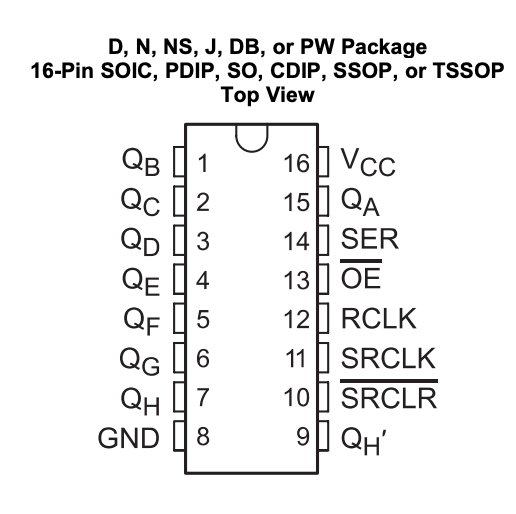
\includegraphics[width=0.5\linewidth]{figures/SN74HC595N.png}}
		\caption{Pin-out diagram van SN74HC595N}
		\label{fig:SN74HC595N}
	\end{figure}

\newpage
\section{Neopixel}
	\paragraph{Probleem:} Je wilt de neopixel (RGB LED) op het bordje gebruiken.
	\paragraph{Oplossing:} CircuitPython heeft een speciale bibliotheek voor het gebruik van de neopixel. Code om de RGB over te laten springen van rood naar groen naar blauw is hieronder te zien.
	\lstinputlisting{code/Neopixel.py}
	
	\paragraph{Discussie:} Zorg er eerst voor dat de neopixel bibliotheek in de lib folder op je bordje staat. Om vervolgens gebruik te maken van de neopixel bibliotheek moet de bibliotheek eerst worden ge\"importeerd. Vervolgens kan gebruik gemaakt worden van de NeoPixel() functie om een NeoPixel object te maken dat controle geeft over de NeoPixel via simpele commando's in de code. De NeoPixel() functie heeft als eerste parameter de I/O pin waar de neopixel op aangesloten is en als tweede parameter het aantal neopixels. In ons geval zit \'e\'en neopixel aangesloten op een interne pin met de naam board.NEOPIXEL. Na het cre\"eren van een neopixel object met de naam 'led', kan de neopixel heel makkelijk worden ingesteld door led aan te roepen in de code. De felheid kan worden ingesteld door led.brightness aan te passen en de kleur van de neopixel kan worden ingesteld door de verhouding van rood/groen/blauw licht in te stellen. Dit kan door elk van de kleuren een waarde tussen de 0 en 255 te geven.
	
	
	\paragraph{Extra informatie over het gebruik van de neopixel}:\\
	
	\url{https://learn.adafruit.com/circuitpython-essentials/circuitpython-internal-rgb-led}
	\url{https://circuitpython.readthedocs.io/projects/neopixel/en/latest/}
	
\section{LCD Screen}
\paragraph{Probleem:} Je wilt tekst naar een LCD screen printen.
\paragraph{Benodigdheden:}
	\begin{itemize}
		\item 1x Bi-Directional Level-Shifter 5-3.3V (Niet nodig maar zorgt voor feller licht)
		\item 1x LCD scherm
		\item 1x PCF8574 i2c LCD controller
	\end{itemize}
\paragraph{Oplossing}:
\begin{figure}[!htb]
	\center{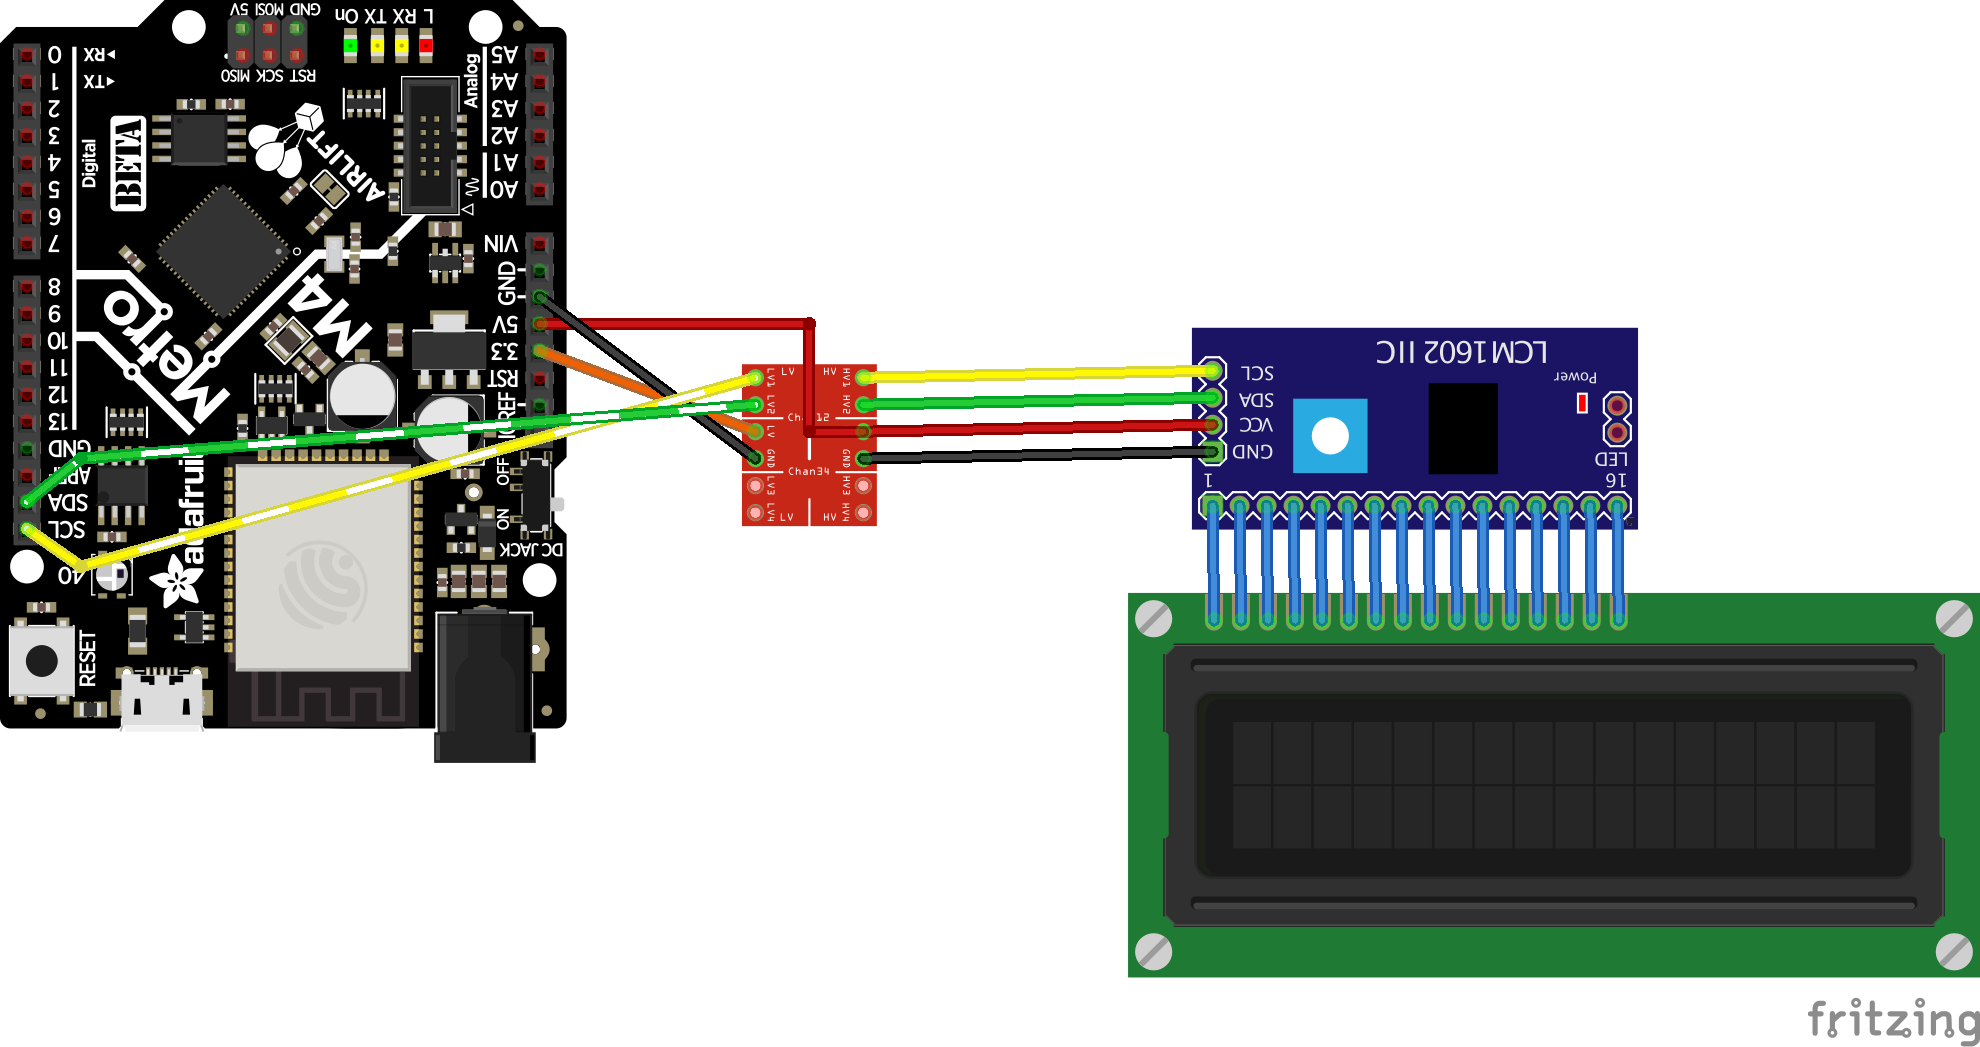
\includegraphics[width=\linewidth]{figures/LCD.png}}
	\caption{LCD Screen Circuit}
	\label{fig:LCD}
\end{figure}
\lstinputlisting{code/LCD.py}
\newpage
\paragraph{Discussie:} Tussen het LCD scherm en het CircuitPython bordje zit een level shifter, omdat het lcd scherm 5V logic gebruikt en het bordje 3.3V. De level shifter heeft een HV en LV pin, waarop de referentie spanning gezet moet worden. Zet op LV dus 3.3V en op HV 5V. De level shifter converteert dan automatisch een spanning van 3.3V op de pinnen LV1-LV4 naar een spanning van 5V op respectivelijk HV1-HV4. De level shifter werkt ook in de andere richting.

Download voor het gebruik van de code eerst de LCD bibliotheek van \url{https://github.com/dhalbert/CircuitPython_LCD} door op \textit{clone or download} en dan \textit{download ZIP} te klikken. Unzip de .zip file en zet het mapje met de naam 'lcd' in de lib folder op je CircuitPython bordje. In de code worden eerst de benodigde modules ge\"importeerd. Daarna wordt een LCD object gemaakt met de naam "lcd". De positie van de cursor kan verplaatst worden met object.set\_cursor\_pos() en er kan tekst geprint worden met object.print(). Met object.clear() wordt het scherm leeg gemaakt en wordt de cursor positie terug naar het begin verplaatst. \\

\clearpage
\newpage

Doet de bibliotheek het niet ? \\

Pas dan de bibliotheek als volgt aan:

\begin{lstlisting}
    def _write4bits(self, value):
        """Pulse the `enable` flag to process value."""
        with self.i2c_device:
            self._i2c_write(value & ~PIN_ENABLE)
            # This 1us delay is probably unnecessary, given the time needed
            # to execute the statements.
            microcontroller.delay_us(1)
            self._i2c_write(value | PIN_ENABLE)
            microcontroller.delay_us(1)
            self._i2c_write(value & ~PIN_ENABLE)
        # Wait for command to complete.
        microcontroller.delay_us(100)
\end{lstlisting}

Voor het volgende stukje code:

\begin{lstlisting}
    def _write4bits(self, value):
        """Pulse the `enable` flag to process value."""
        with self.i2c_device:
            self._i2c_write(value & ~PIN_ENABLE)
            # This 1us delay is probably unnecessary, given the time needed
            # to execute the statements.
            #microcontroller.delay_us(1)
            self._i2c_write(value | PIN_ENABLE)
            #microcontroller.delay_us(1)
            self._i2c_write(value & ~PIN_ENABLE)
        # Wait for command to complete.
        #microcontroller.delay_us(100)
\end{lstlisting}
	\chapter{Sensoren}
Informatie over de buitenwereld krijg je door middel van sensoren. Sensoren zijn er in allerlei soorten en maten, maar werken vaak op hetzelfde principe. Een fysische gebeurtenis wordt geconverteerd naar een elektrisch signaal dat kan worden verwerkt door de microprocessor. Dit hoofdstuk bevat recepten voor het uitlezen van een aantal sensoren.

\newpage
\section{Potentiometer}
\paragraph{Probleem:} Je wilt een potentiometer uitlezen.
\paragraph{Benodigdheden:}
\begin{itemize}
	\item 1x Potentiometer
	\item 1x \SI{4.7}{\kilo\ohm} weerstand
\end{itemize}
\paragraph{Oplossing:}
\begin{figure}[H]
	\center{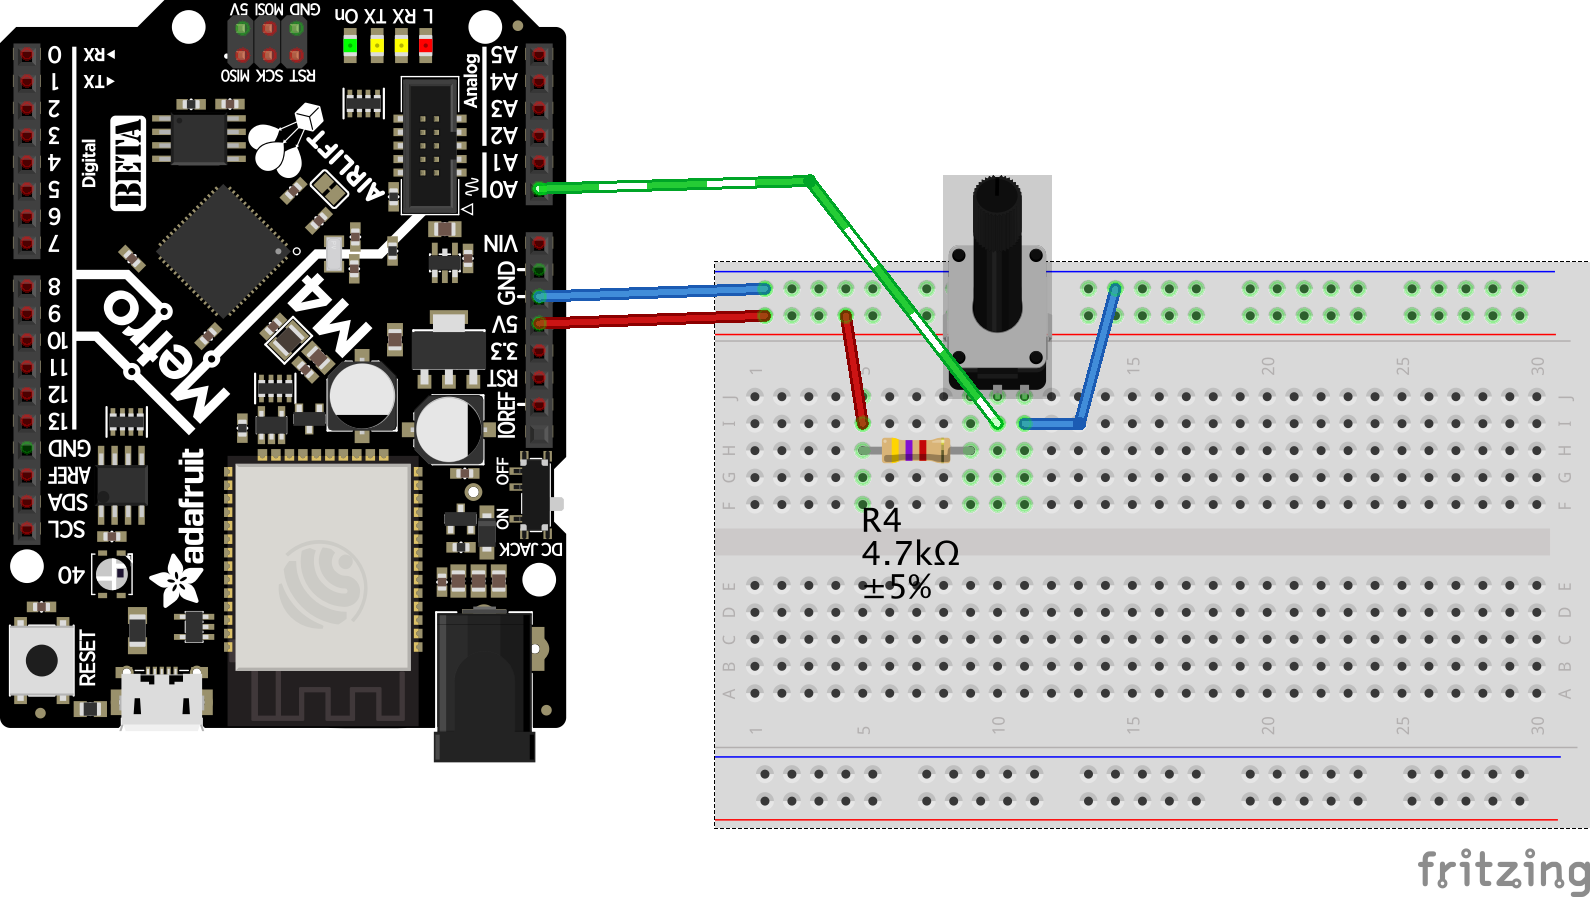
\includegraphics[width=\linewidth]{figures/PotSensor.png}}
	\caption{Potentiometer Sensor Circuit}
	\label{fig:PotSensor}
\end{figure}
\lstinputlisting{code/Lightsensor_TEMT6000.py}
\paragraph{Discussie:} Een potentiometer is een variabele spanningsdeler. Een potentiometer verbindt zowel de eerste pin en tweede pin met een weerstand als de tweede en derde pin met een weerstand. Door aan de potentiometer te draaien verander je de verhouding tussen de 2 weerstanden. Een potentiometer van \SI{10}{\kilo\ohm} heeft wel altijd een totale weerstand van \SI{10}{\kilo\ohm} tussen de eerste en derde pin. Door aan de pin te draaien kan je de verhouding wel veranderen in bijvoorbeeld \SI{1}{\kilo\ohm} tussen pin 1 en 2 en \SI{9}{\kilo\ohm} tussen pin 2 en 3 of \SI{0}{\kilo\ohm} tussen 1 en 2 en \SI{10}{\kilo\ohm} tussen 2 en 3.  Als \SI{3.3}{\volt} op pin 1 staat en pin 3 verbonden is met ground verandert de spanning op pin 2 evenredig meet de stand van de potentiometer. Omdat de tweede pin van de potentiometer in dit circuit direct zit aangesloten op een I/O pin, wordt een extra resistor toegevoegd om een short-circuit te voorkomen. Dit kan gebeuren in het geval dat de weerstand tussen pin 1 en pin 2 \SI{0}{\ohm} is.

Voor het uitlezen van een analoog signaal heeft CircuitPython de analogio bibliotheek. In de code hoef je alleen een object te maken door het analoge pin nummer als parameter aan de AnalogIn() functie te geven. De waarde van de spanning op de pin kan dan uitgelezen worden door objectnaam.value aan te roepen in de code.  De analoge waarde wordt uitgedrukt in een 16-bit digitaal getal. Een 16-bit digitaal getal kan 65536 waarden representeren, de waarden 0-65535. De waarde 0 wordt uitgelezen als een spanning van \SI{0}{\volt} op de pin wordt gezet en de waarde 65535 als een spanning van \SI{3.3}{\volt} op de pin wordt gezet. Om het digitale getal te converteren naar de analoge spanning wordt in de gedefinieerde get\_voltage() functie de uitgelezen waarde gedeeld door het aantal mogelijke nummers en vermenigvuldigd met 3.3. In de while loop wordt vervolgens elke tiende seconde de waarde geprint. Open ook de \textbf{plotter} in Mu editor om de waarden in de grafiek te zien veranderen als je aan de potmeter draait.

\newpage
\section{Een licht aan en uit zetten op basis van de licht intensitiet}
	\paragraph{Probleem:} Je wilt een automatisch licht dat aangaat als het donker wordt.
	\paragraph{Benodigdheden:}
	\begin{itemize}
		\item 1x LED
		\item 1x \SI{680}{\ohm} weerstand
		\item 1x TEMT6000 lichtsensor
	\end{itemize}
	\paragraph{Oplossing}:	
		\begin{figure}[H]
			\center{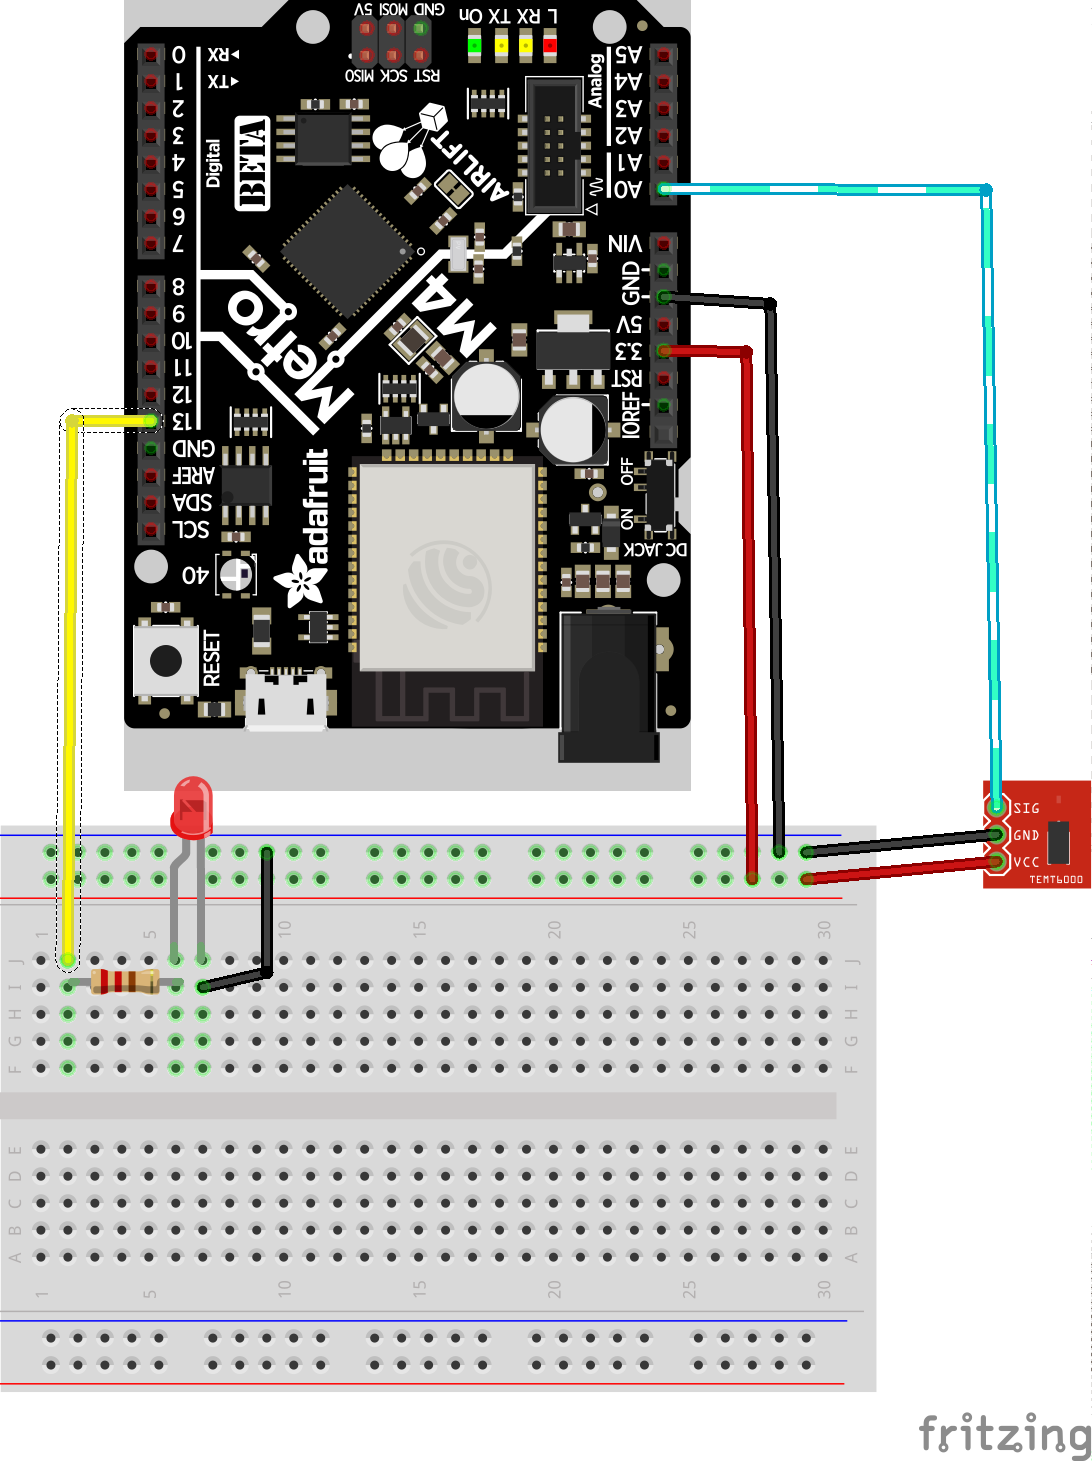
\includegraphics[width=0.6\linewidth]{figures/LightSensor_TEMT6000.png}}
			\caption{TEMT6000 lightsensor circuit}
			\label{fig:Lightsensor}
		\end{figure}
\newpage
		\lstinputlisting{code/Lightsensor_TEMT6000_OnOff.py}
	\paragraph{Discussie:} De lichtsensor is een analoge sensor waar een spanning uitkomt die evenredig is met de lichtintensiteit. De werking van een lichtsensor is vergelijkbaar met dat van een potentiometer, beide werken met het principe van een spanningsdeler. In het geval van een lichtsensor is het alleen niet een mechanische draaiknop dat de verhouding tussen de weerstanden verandert, maar de lichtintensiteit. De code om de spanning van de lichtsensor uit te lezen is precies hetzelfde als bij de potentiometer. De analogio module wordt ge\"importeerd en uitgelezen met de get\_voltage() functie. In dit geval wordt niet alleen de waarde van de sensor uitgelezen, maar wordt ook een LED aangezet als de lichtintensiteit een sensor spanning lager dan \SI{1.65}{\volt} geeft.
	

\newpage	
\section{Een licht feller laten branden als het donkerder wordt.}
    \paragraph{Probleem:} Je wilt de felheid van een ledje aanpassen op de intensiteit van het licht.
    \paragraph{Benodigdheden:}
    \begin{itemize}
    	\item 1x LED
    	\item 1x \SI{680}{\ohm} weerstand
    	\item 1x TEMT6000 lichtsensor
    \end{itemize}
    \paragraph{Oplossing:} Circuit in Figuur~\ref{fig:Lightsensor}
		\lstinputlisting{code/Lightsensor_TEMT6000_PWM.py}
	\paragraph{Discussie:}
		Dit is een variatie op het aan en uitzetten van de lichtsensor. Hier wordt \textbf{P}ulse-\textbf{W}idth \textbf{M}odulation gebruikt om het ledje feller en minder fel te maken op basis van de lichtintensiteit. De pulseio module wordt ge\"importeerd om PWM te gebruiken. In plaats van een DigitalInOut wordt nu een PWMout object gemaakt met de naam 'pwm' die geassocieerd is met pin D13. De intensiteit van de LED kan nu geregeld worden door de waarde pwm.duty\_cycle te veranderen. Ook PWM heeft een waarde tussen 0 en 65535, net als het uitlezen van een analoog signaal. De duty\_cycle is lineair gerelateerd aan het voltage uit de pin. Een waarde van 0 zet een spanning van 0V op de I/O pin en 65535 een waarde van 3.3V. In de code wordt een spanning van 3.3V op de pwm pin gezet als een lichtintensiteit van 0V wordt gemeten, 1.65V als 1.65V wordt gemeten en 0V als een spanning van 3.3V wordt gemeten.






\newpage
\section{Ultrasone afstandssensor}
	\paragraph{Probleem:} Je wilt de afstand tot een object meten met een ultrasone sensor.
	\paragraph{Benodigdheden:}
	\begin{itemize}
		\item 1x HCSR04 Ultrasone afstandssensor
	\end{itemize}
	\paragraph{Oplossing}:
	\begin{figure}[H]
		\center{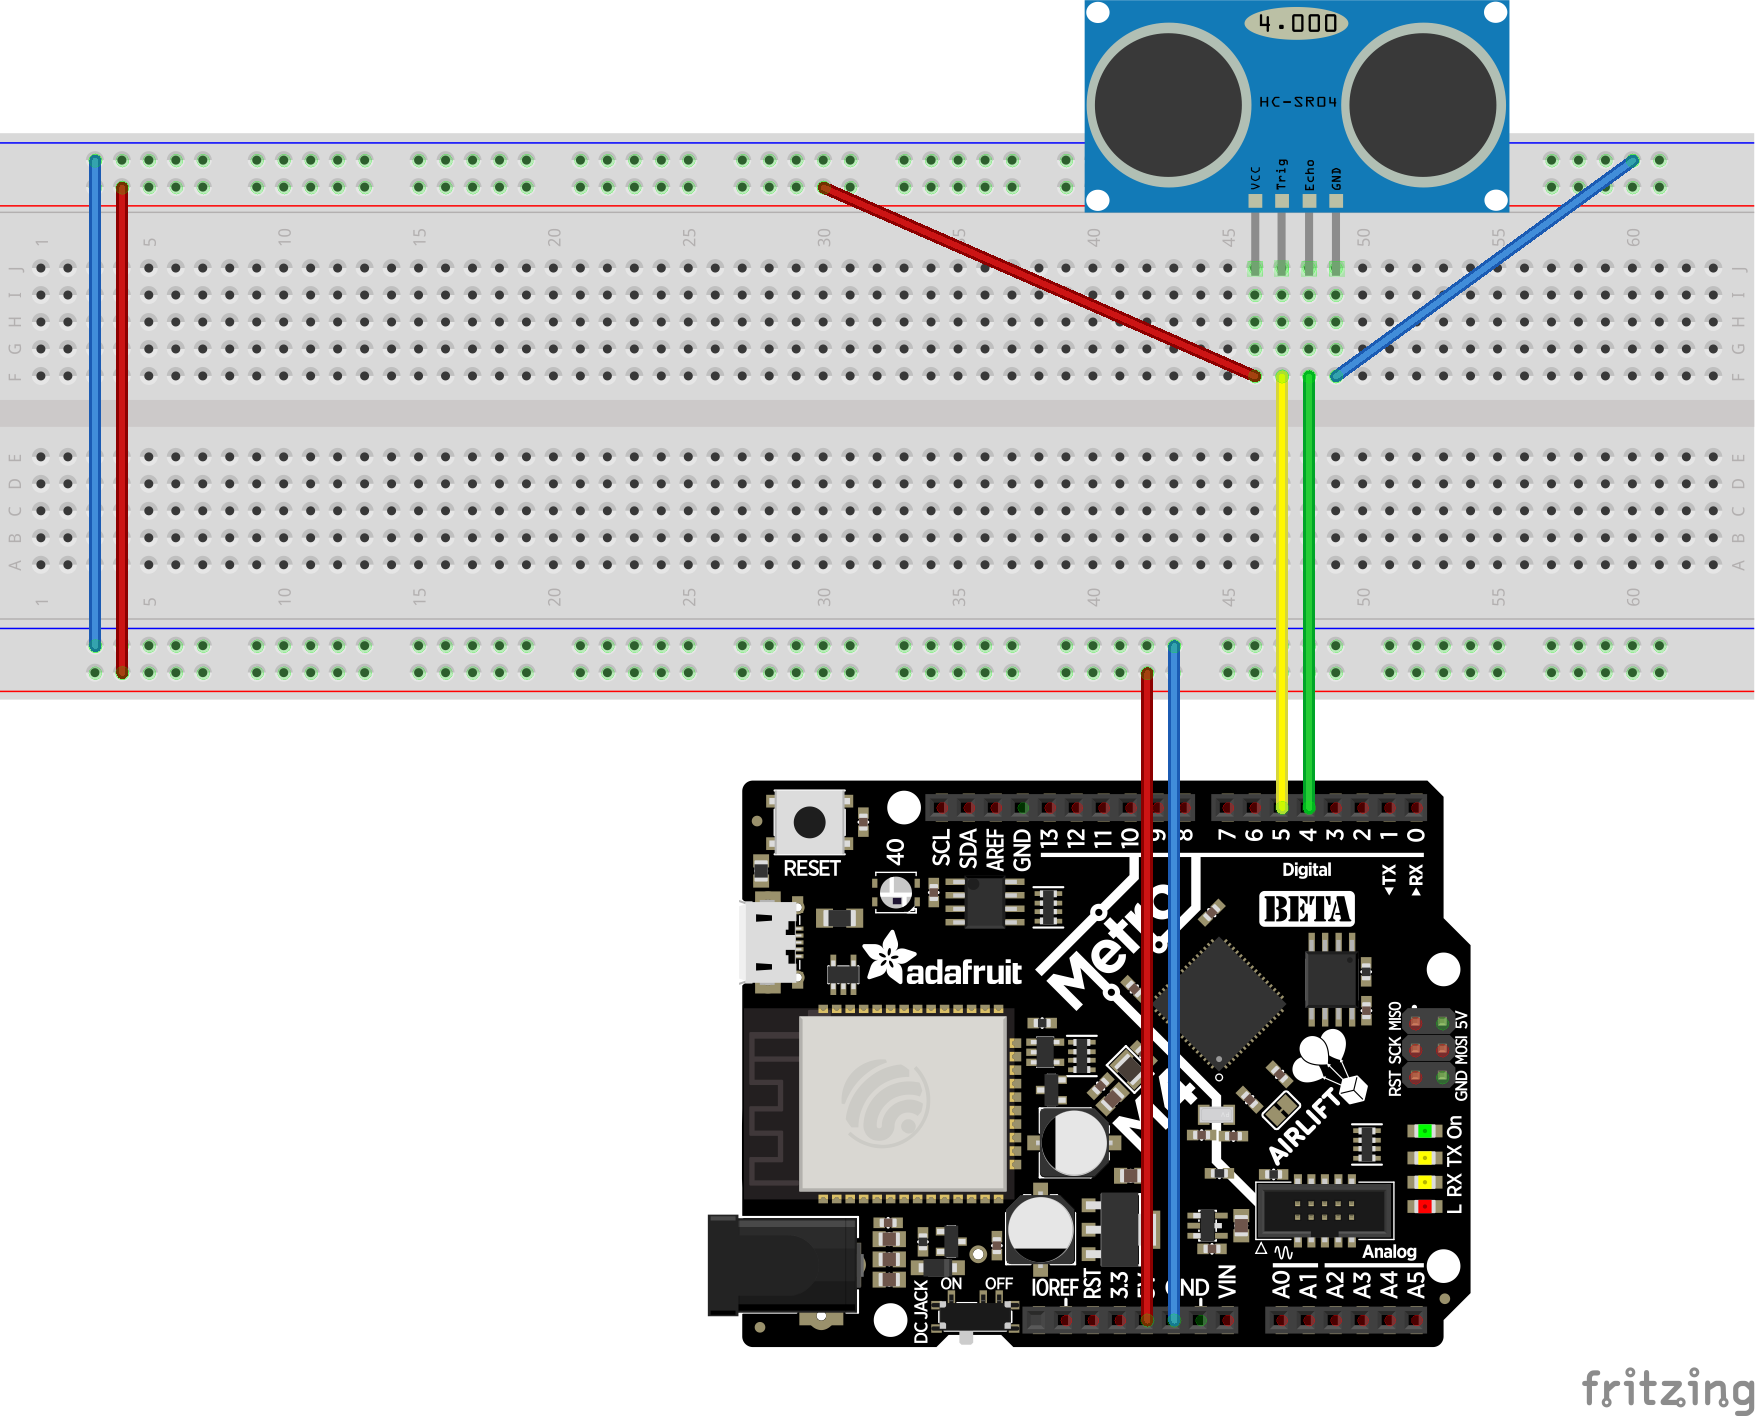
\includegraphics[width=0.6\linewidth]{figures/UltrasonicDistance.png}}
		\caption{Ultrasonic Distance Circuit}
		\label{fig:UltrasonicDistance}
	\end{figure}

%\newpage
	\lstinputlisting{code/UltrasonicDistance.py}
	\newpage
	
	\paragraph{Discussie:} Voor het gebruik van een ultrasone afstandssensor hoef je zelf weinig te programmeren, want Adafruit heeft hier een speciale bibliotheek voor in hun CircuitPython library bundel. Deze bundel kan je vinden op \url{https://circuitpython.org/libraries}. Zorg dat het adafruit\_hcsr04.mpy bestand in de lib folder op je bordje staat. 
	
	In de code hoef je nu alleen de adafruit\_hcsr04 te importeren en een nieuw object te maken met de HCSR04 functie, waarin je de trigger en echo pin nummers moet geven als parameters. Dit object krijgt in de code de naam sonar. De afstand kan nu eenvoudig gemeten worden door sonar.distance aan te roepen. Dit wordt in de code gedaan in een try/except block. Dit voorkomt dat de code crasht als er een runtime error optreedt bij het aanroepen van sonar.distance.
	
\newpage
\section{Joystick}
	\paragraph{Probleem:} Je wilt een joystick uitlezen en gebruiken in een project. 
	\paragraph{Benodigdheden:}
	\begin{itemize}
		\item 1x Joystick
	\end{itemize}
	\paragraph{Oplossing}:
		\begin{figure}[H]
			\center{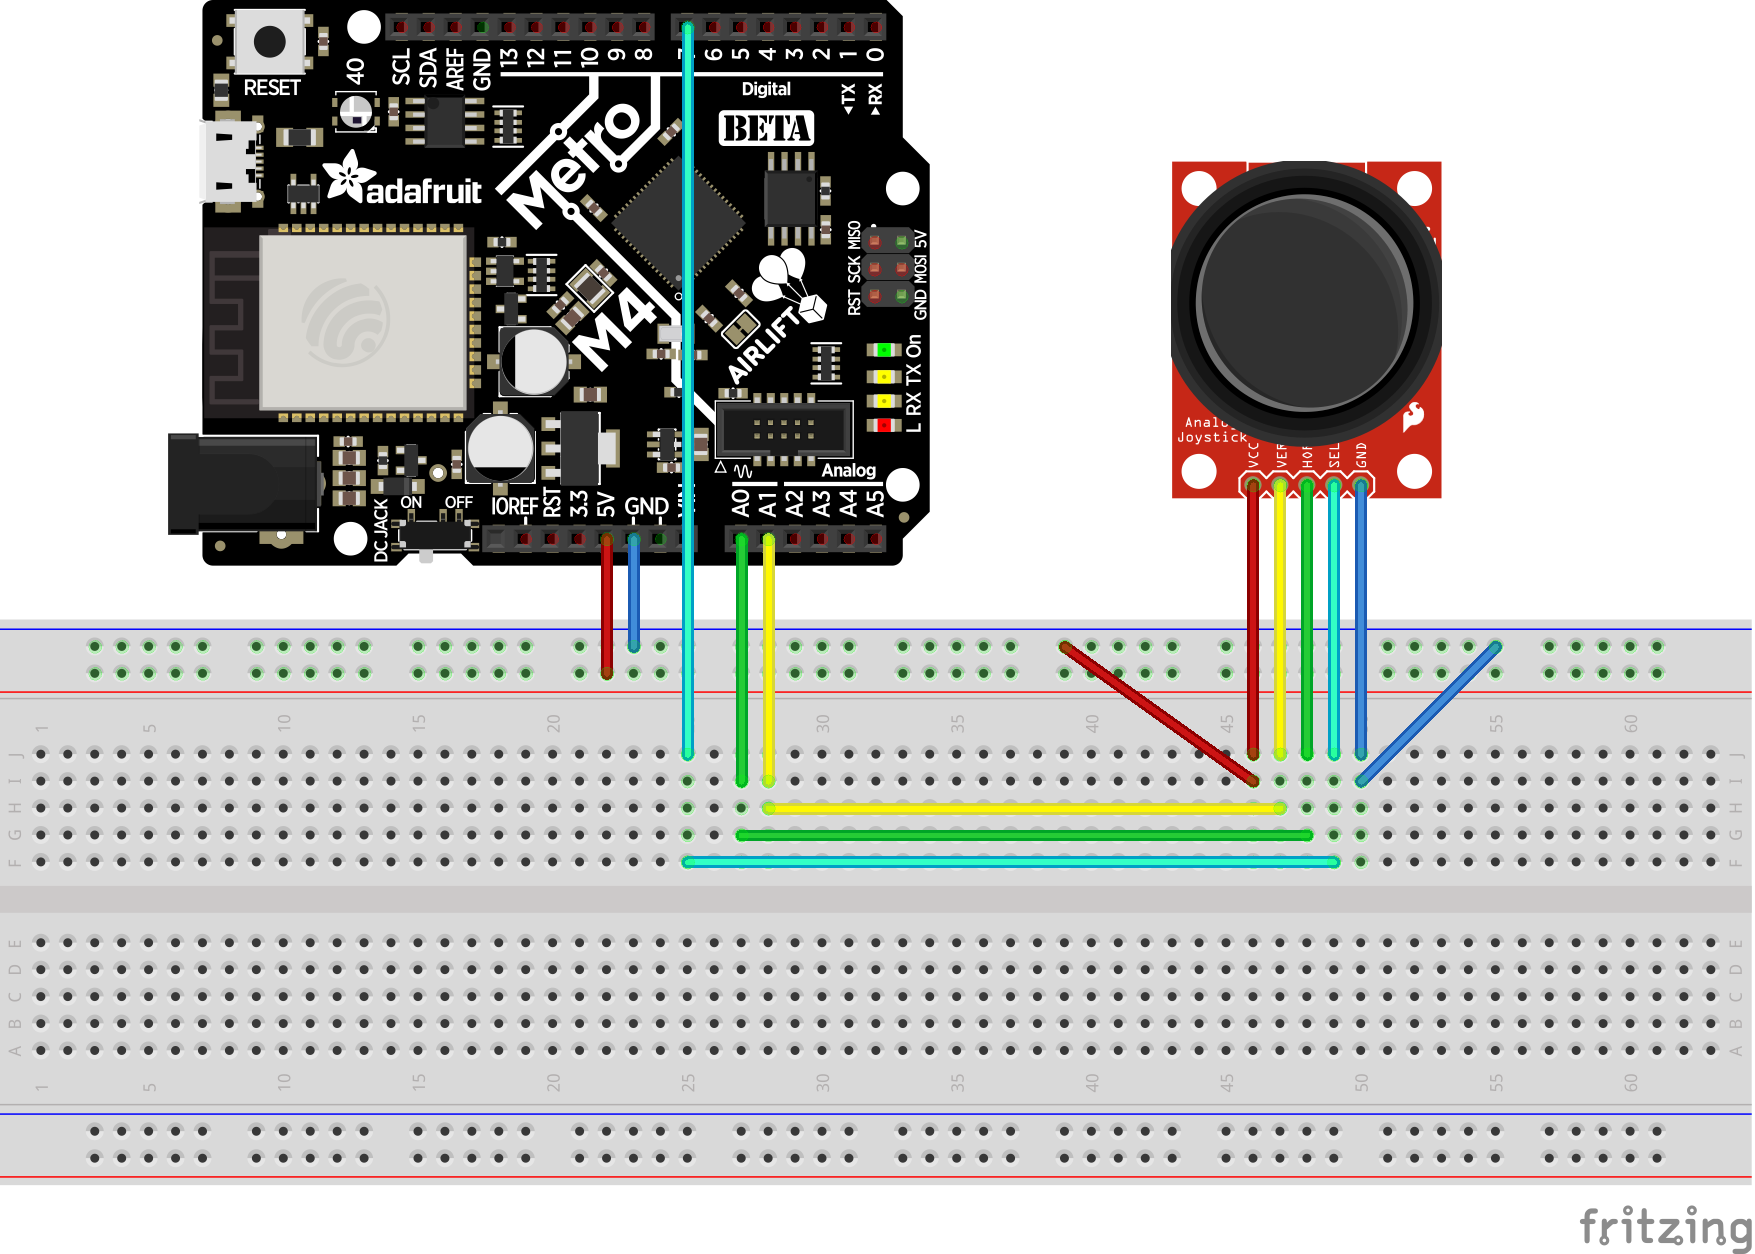
\includegraphics[width=0.8\linewidth]{figures/Joystick.png}}
			\caption{Joystick Circuit}
			\label{fig:Joystick}
		\end{figure}
	\newpage
		\lstinputlisting{code/Joystick.py}
	\paragraph{Discussie:} Een joystick bestaat uit 2 analoge potentiometers en 1 digitale knop. De benodigde modules voor het uitlezen van de joystick zijn de board, time, digitalio en analogio module.\\
	
	Links/rechts wordt uitgelezen op A1, omhoog/omlaag op A0 en het indrukken op D7.  De richting van D7 wordt op input gezet en een pull-up weerstand wordt gebruikt om de pin hoog te houden zolang de knop niet wordt ingedrukt. Als geen pull-up weerstand zou worden gebruikt, dan is niet bekend wat de waarde van de input is als de knop niet wordt ingedrukt. Het kan dan gebeuren dat de uitgelezen spanning dichter bij ground zit dan bij \SI{3.3}{\volt} en wordt dan uitgelezen alsof de knop wordt ingedrukt, terwijl dit niet gebeurd. Pull-up en pull-down weerstanden worden gebruikt om deze 'zwevende' waarden een vaste waarde te geven. \\
	
	In de oneindige while loop wordt elke tiende seconde eerst gekeken of de knop van de joystick is ingedrukt. Als dit niet zo is worden de 2 spanningen geprint. Als de knop wel wordt ingedrukt wordt "button pressed" geprint. Open ook de \textbf{plotter} in mu editor om de waarden te zien veranderen als je de joystick beweegt. 
	
	

\newpage
\section{RC Lowpass Filter}
	\paragraph{Probleem:} Je wilt het effect van een low-pass filter zien.
	\paragraph{Benodigdheden:}
	\begin{itemize}
		\item 1x \SI{15}{\kilo\ohm} weerstand
		\item 1x \SI{10}{\micro\farad} condensator
	\end{itemize}
	\paragraph{Oplossing}:
	\begin{figure}[H]
		\center{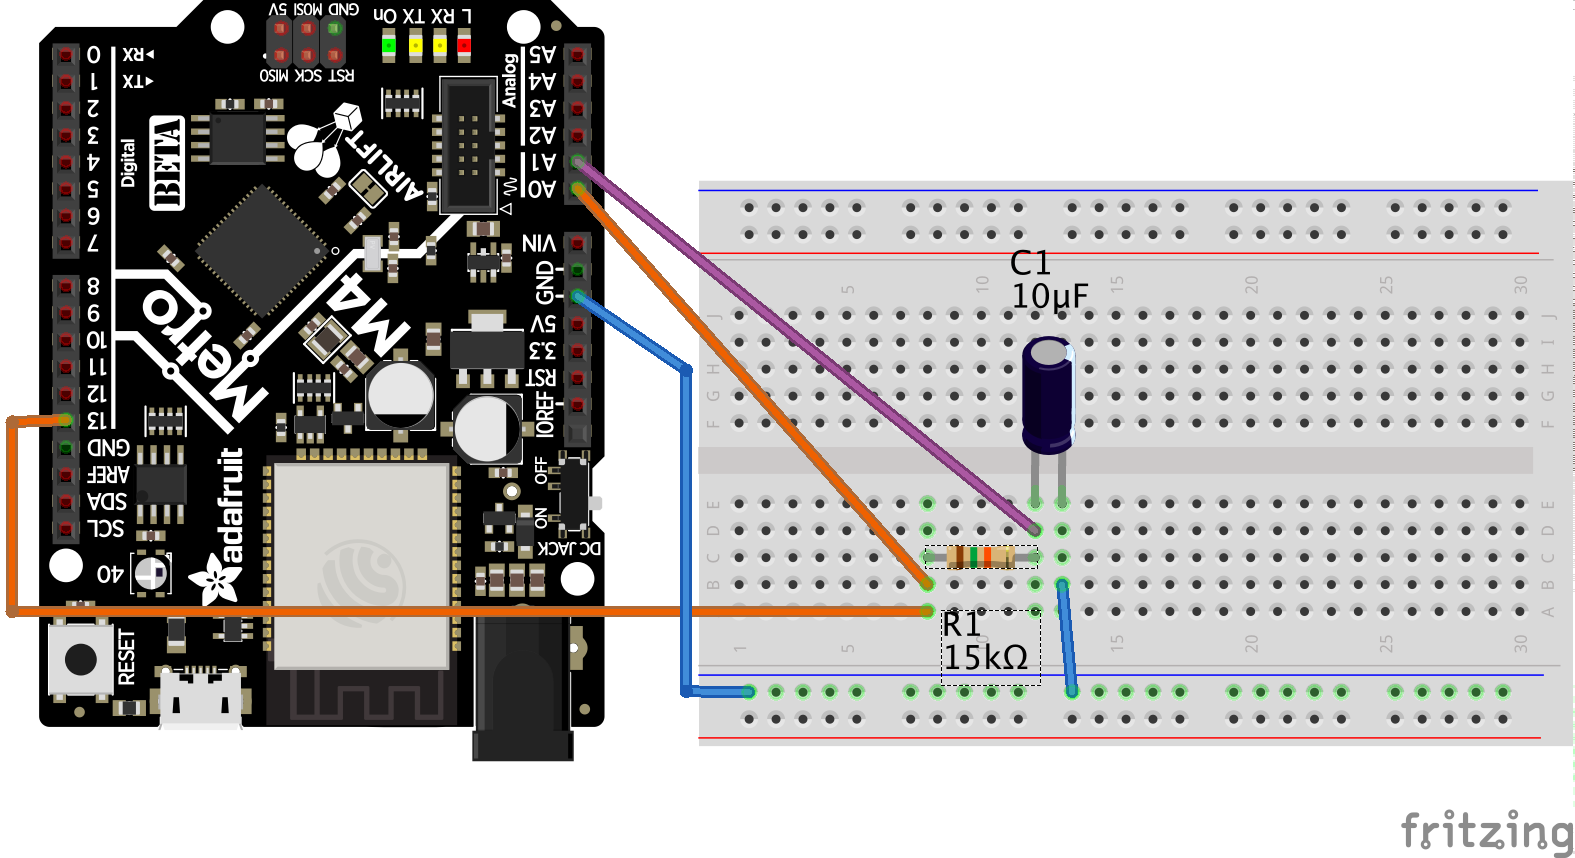
\includegraphics[width=0.8\linewidth]{figures/RC_Filter_PWM.png}}
		\caption{RC-filter Circuit}
		\label{fig:PWM_Filter}
	\end{figure}
	
	\newpage
	\lstinputlisting{code/PWM_Filter.py}
	\paragraph{Discussie:} Een \textbf{R}esistor \textbf{C}apacitor low-pass filter wordt gebruikt om hoge frequenties in signalen weg te filteren en lage frequenties door te laten. Low-pass filters worden vaak gebruikt om ruis uit sensor signalen te halen, maar ook door bijvoorbeeld dj's om hoge frequenties uit muziek te filteren. Om inzicht te krijgen in het effect van een RC-filter wordt in dit recept een PWM blokgolf gebruikt, die zowel gefilterd als ongefilterd wordt uitgelezen door een analoge input. \\
	
	De time, board, pulseio en analogio modules worden eerst ge\"importeerd. Er worden 2 analoge inputs ge\"initialiseerd op A0 en A1 en er wordt een PWM signaal  met een frequentie van 1 Hz en een duty cycle van 0.5 op pin D13 ge\"initaliseerd. \'E\'en signaal gaat direct van de PWM output naar A0. Dit signaal is ongefilterd. Het andere signaal gaat eerst door de RC filter voordat het bij A1 aankomt. De outputs worden vervolgens elke honderdste seconde geprint. Open de plotter in mu editor om de verschillende signalen te zien.
	
	
	\chapter{Aandrijving}
De combinatie van het uitlezen van sensoren met het aandrijven van hardware vormt de basis van alle meet- en regel systemen. Dit hoofdstuk bevat recepten voor het aansturen van hardware.

\section{Transistors}
\paragraph{Probleem:}
Je wilt een systeem aansturen dat meer power nodig heeft dan je I/O pinnen kunnen leveren, zie hoofdstuk~\ref{sec:VeiligOmgaan}. Door middel van een transistor kan het circuit, net als met een schakelaar, open en gesloten worden. Een I/O pin stuurt deze 'schakelaar' aan, terwijl een externe bron de stroom levert.

\paragraph{Benodigdheden:}
\begin{itemize}
	\item 1x LED
	\item 1x \SI{100}{\ohm} weerstand
	\item 1x \SI{3.9}{\kilo\ohm} weerstand
	\item 1x NPN transistor (BJT)
\end{itemize}

\paragraph{Oplossing}: 

	\begin{figure}
		\center{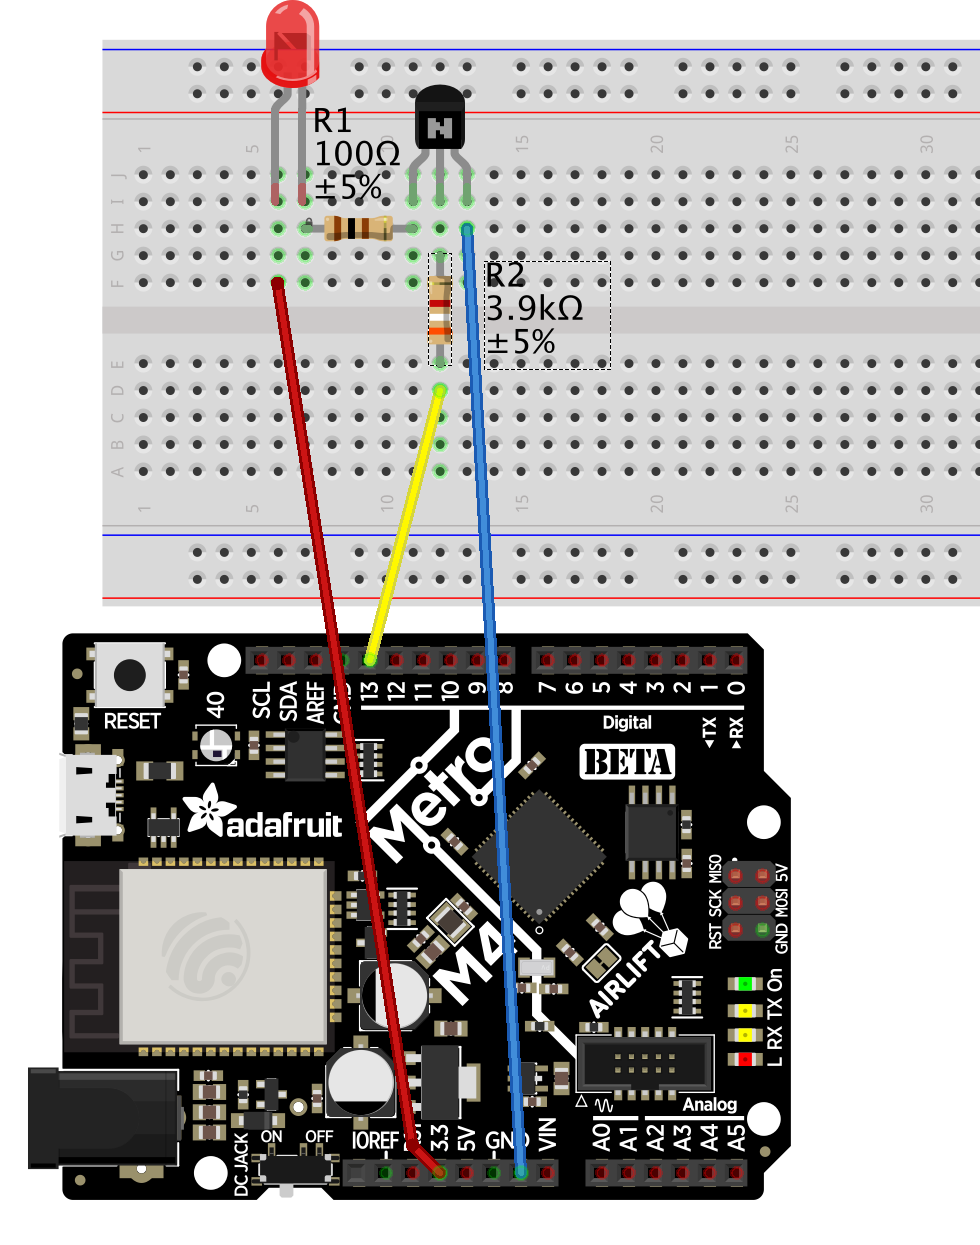
\includegraphics[width=0.5\linewidth]{figures/TransistorLED.png}}
		\caption{Transistor Circuit}
		\label{fig:TransistorLED}
	\end{figure}

\paragraph{Transistor Berekening:}
\begin{figure}
	\center{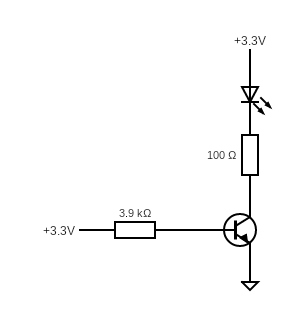
\includegraphics[width=0.6\linewidth]{figures/Transistorcircuit.png}}
	\caption{Transistor Diagram}
	\label{fig:TransistorDiagram}
\end{figure}

\begin{alignat}{9}
\beta &\approx 25\to 100\\
V_{source}&=\SI{3.3}{\volt}\\
V_{CE}&=\SI{0.1}{\volt}\\
V_{BE}&=\SI{0.8}{\volt}\\
V_{LED}&=\SI{2}{\volt}\\
I_{C_{Verzadigd}}&=\SI{12}{\milli\ampere}\\
I_B&>\frac{I_{C_{SAT}}}{25}=\SI{0.48}{\milli\ampere}\\
R_C& \approx \frac{V_{source}-V_{CE}-V_{LED}}{I_{C_{SAT}}} \approx \SI{100}{\ohm}\\
R_B& < \frac{V_{source}-V_{BE}}{I_B}<\SI{5.2}{\kilo\ohm}
\end{alignat}

\paragraph{Discussie:} Transistors zijn op verschillende manieren te gebruiken. Als versterker of als schakelaar. In dit voorbeeld wordt de transistor als schakelaar gebruikt. Eerst moet bepaald worden hoeveel stroom er door de LED moet. Maximale stroom door een LED is vaak rond de \SI{20}{\milli\ampere}. In dit voorbeeld wordt een veilige stroom van \SI{12}{\milli\ampere} genomen. Op basis van de Collector-Emitter spanningsval(te vinden in de transistor datasheet), de spanningsval over de LED en de bronspanning kan de weerstand in serie met de LED berekend worden. Met deze weerstand is de \SI{12}{\milli\ampere} de maximale stroom die van de collector naar de emitter kan stromen. Dit is dan ook de stroom die loopt als de transistor verzadigd is. Om de transistor als schakelaar te gebruiken en niet als versterker, moet er voor gezorgd worden dat de Base-Emitter stroom hoog genoeg is om de transistor te verzadigen. Dit is afhankelijk van de verzadigde stroom(\SI{12}{\milli\ampere}) en de \textit{gain} of versterking $\beta$. $\beta$ is te vinden in de data sheet en ligt vaak tussen de 25 en 100. Om er zeker van te zijn dat verzadiging bereikt wordt, wordt met een lage versterking van 25 de benodigde base-emitter stroom bepaald. De benodigde base-emitter stroom kan vervolgens samen met de bronspanning en base-emitter spanningsval gebruikt worden om de weerstand aan de base te berekenen.

\newpage



\section{DC Motor}\label{sec:DCMotor}
\paragraph{Probleem:}
Je wilt een DC aansturen met je micro-controller, dat zowel vooruit als achteruit kan draaien.

\paragraph{Benodigdheden:}
\begin{itemize}
	\item 1x 9V batterij
	\item 1x L298N H-Bridge Motor Driver
	\item 1x DC Motor
\end{itemize}

\paragraph{Oplossing}:

	\begin{figure}[H]
		\center{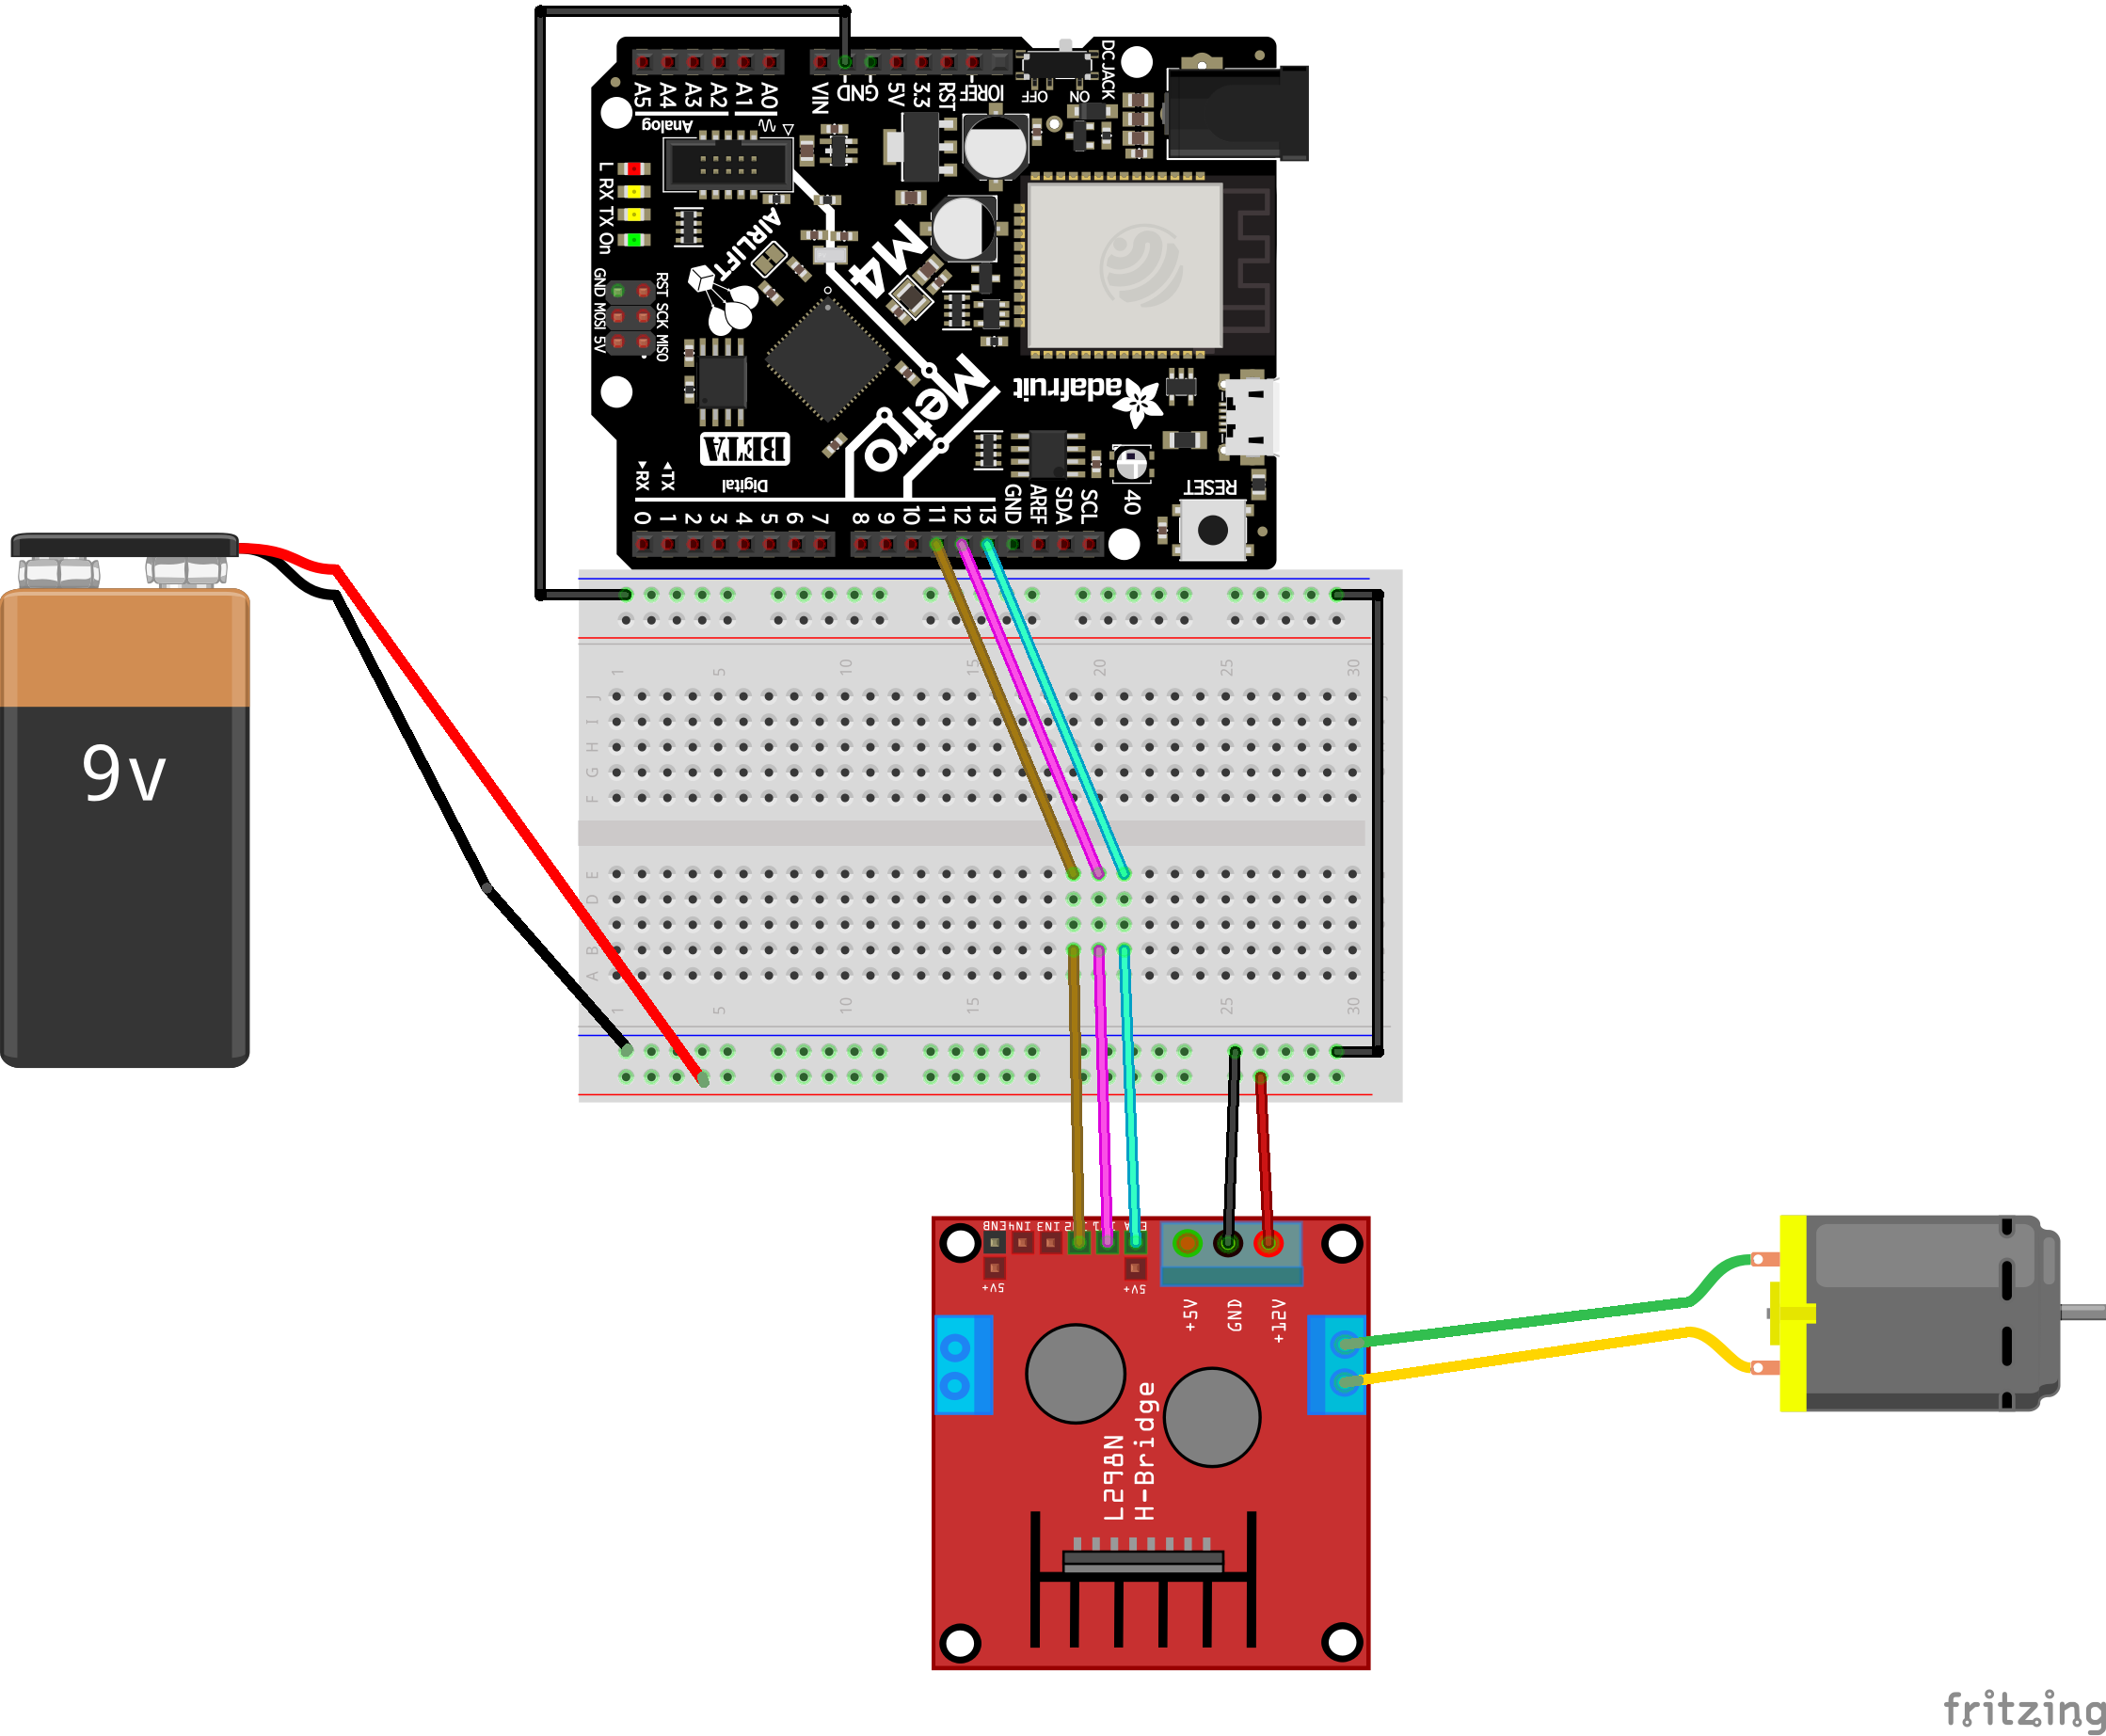
\includegraphics[width=\linewidth]{figures/DC_Motor.png}}
		\caption{MotorDriver Circuit}
		\label{fig:MotorDriver}
	\end{figure}
\newpage
		\lstinputlisting{code/DC_Motor.py}

	

\paragraph{Discussie:} Het bordje kan zelf niet het vermogen leveren voor de motor en met alleen een positieve spanning kan de motor normaal gesproken maar in 1 richting draaien. Met het gebruik van een H-brug kan zowel een externe spanningsbron gebruikt worden als in 2 richtingen gedraaid worden. Met de IN1 en IN2 pinnen op de H-brug kan de richting ingesteld worden door op 1 pin een hoge spanning te zetten en op de ander een lage spanning. Met de ENA pin wordt de motor aan en uit gezet. Door hier een blok golf op te zetten met PWM kan ook de snelheid geregeld worden door de duty cycle aan te passen. 

In de code worden zoals gewoonlijk eerst de benodigde modules geimporteerd. Daarna wordt gedefinieerd welke I/O pinnen zijn aangesloten op de pinnen van de H-brug. De ENA pin wordt geinitaliseerd als PWM, en de IN1 en IN2 als digitale outputs. Er worden ook functies gedefinieerd om de motor vooruit en achteruit te laten draaien, met als input de duty cycle. Allebei de functies werken hetzelfde. Eerst wordt de motor uitgezet, dan wordt de richting bepaald door de IN1 en IN2 pinnen en dan wordt de motor aan gezet met de juiste duty cycle.

De oneindige while loop laat de motor een halve seconde vooruit draaien en daarna een halve seconde achteruit.



\section{Twee DC motoren}\label{sec:TwoDCMotors}
	\paragraph{Probleem:} Je wilt twee DC motoren tegelijkertijd aansturen.
	
	\paragraph{Benodigdheden:}
	\begin{itemize}
		\item 1x 9V batterij
		\item 1x L298N H-Bridge Motor Driver
		\item 2x DC Motor
	\end{itemize}
	
	\paragraph{Oplossing}: 
	\lstinputlisting{code/Two_DC_Motor.py}
	
	\begin{figure}[H]
		\center{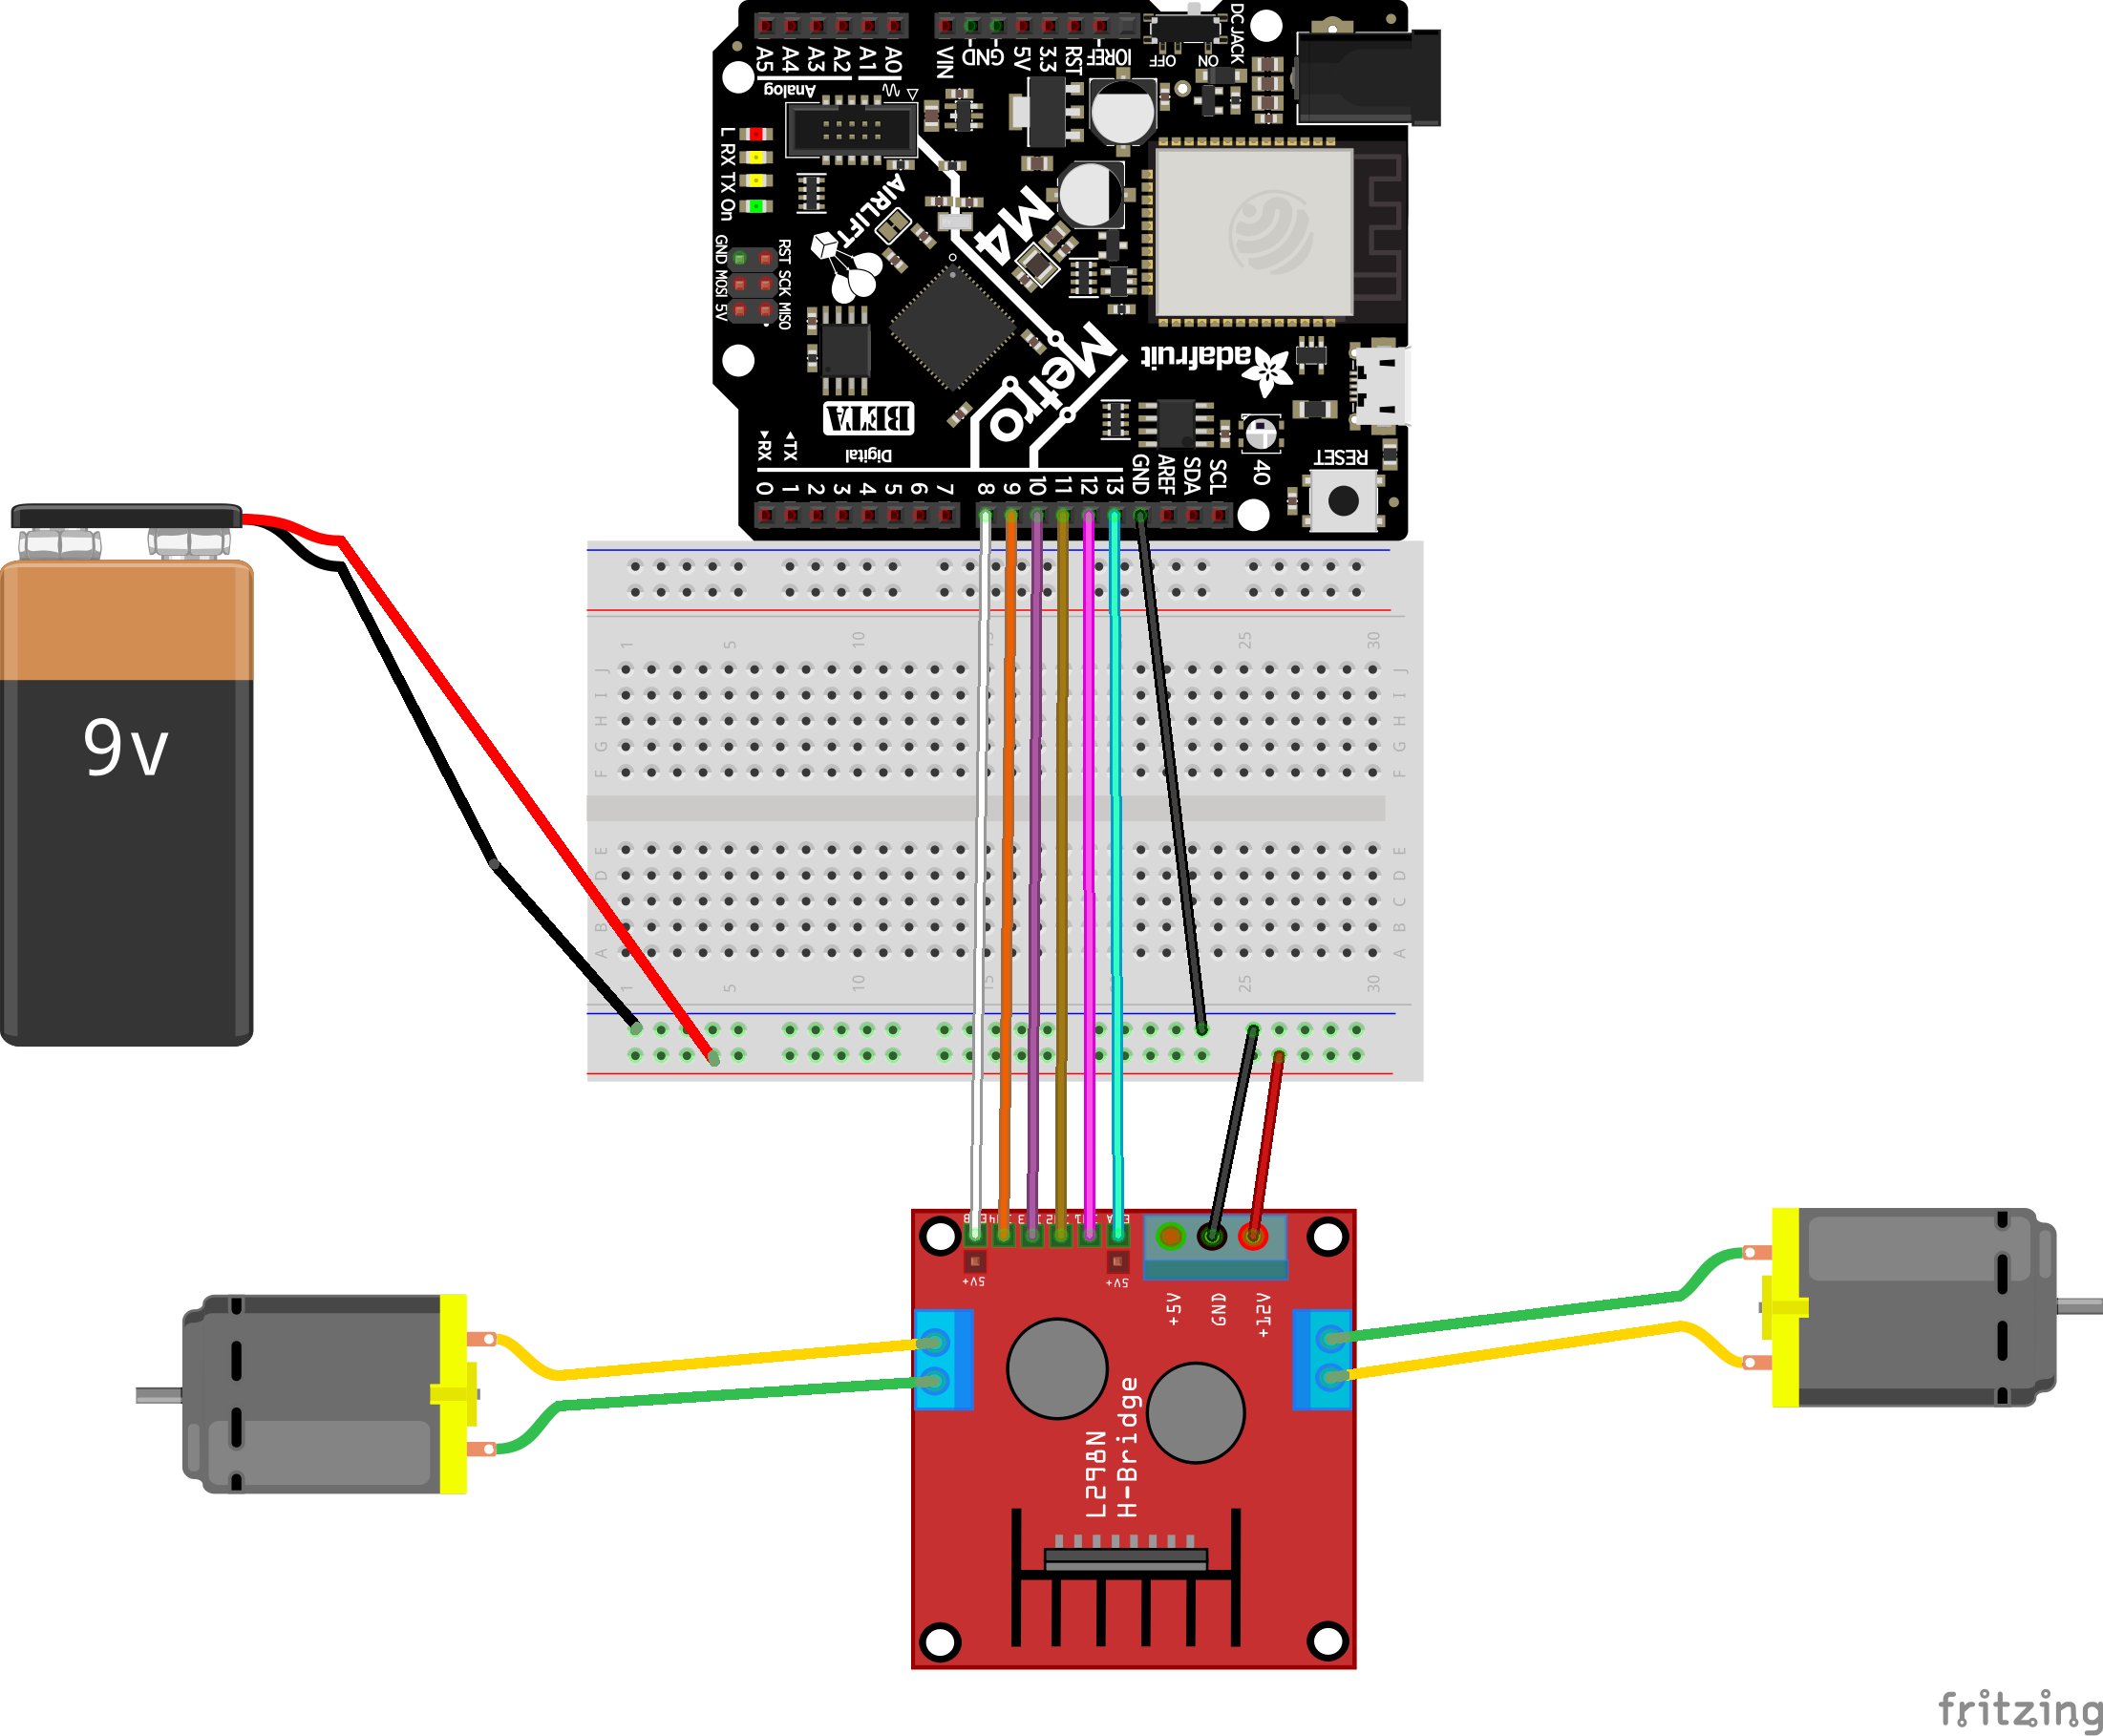
\includegraphics[width=0.8\linewidth]{figures/MotorDriver.png}}
		\caption{Double Motor Driver Circuit}
		\label{fig:Two_DC_Motor}
	\end{figure}

	\paragraph{Discussie:} De code is haast hetzelfde als met 1 DC motor in recept~\ref{sec:DCMotor}, maar alles dubbel gedefinieerd. 
	
\newpage
\section{Servo}\label{sec:servo}
\paragraph{Probleem:} Je wilt een Servo aansturen.

\paragraph{Benodigdheden:}
\begin{itemize}
	\item 1x Servo
\end{itemize}

\paragraph{Oplossing}:

\begin{figure}[H]
	\center{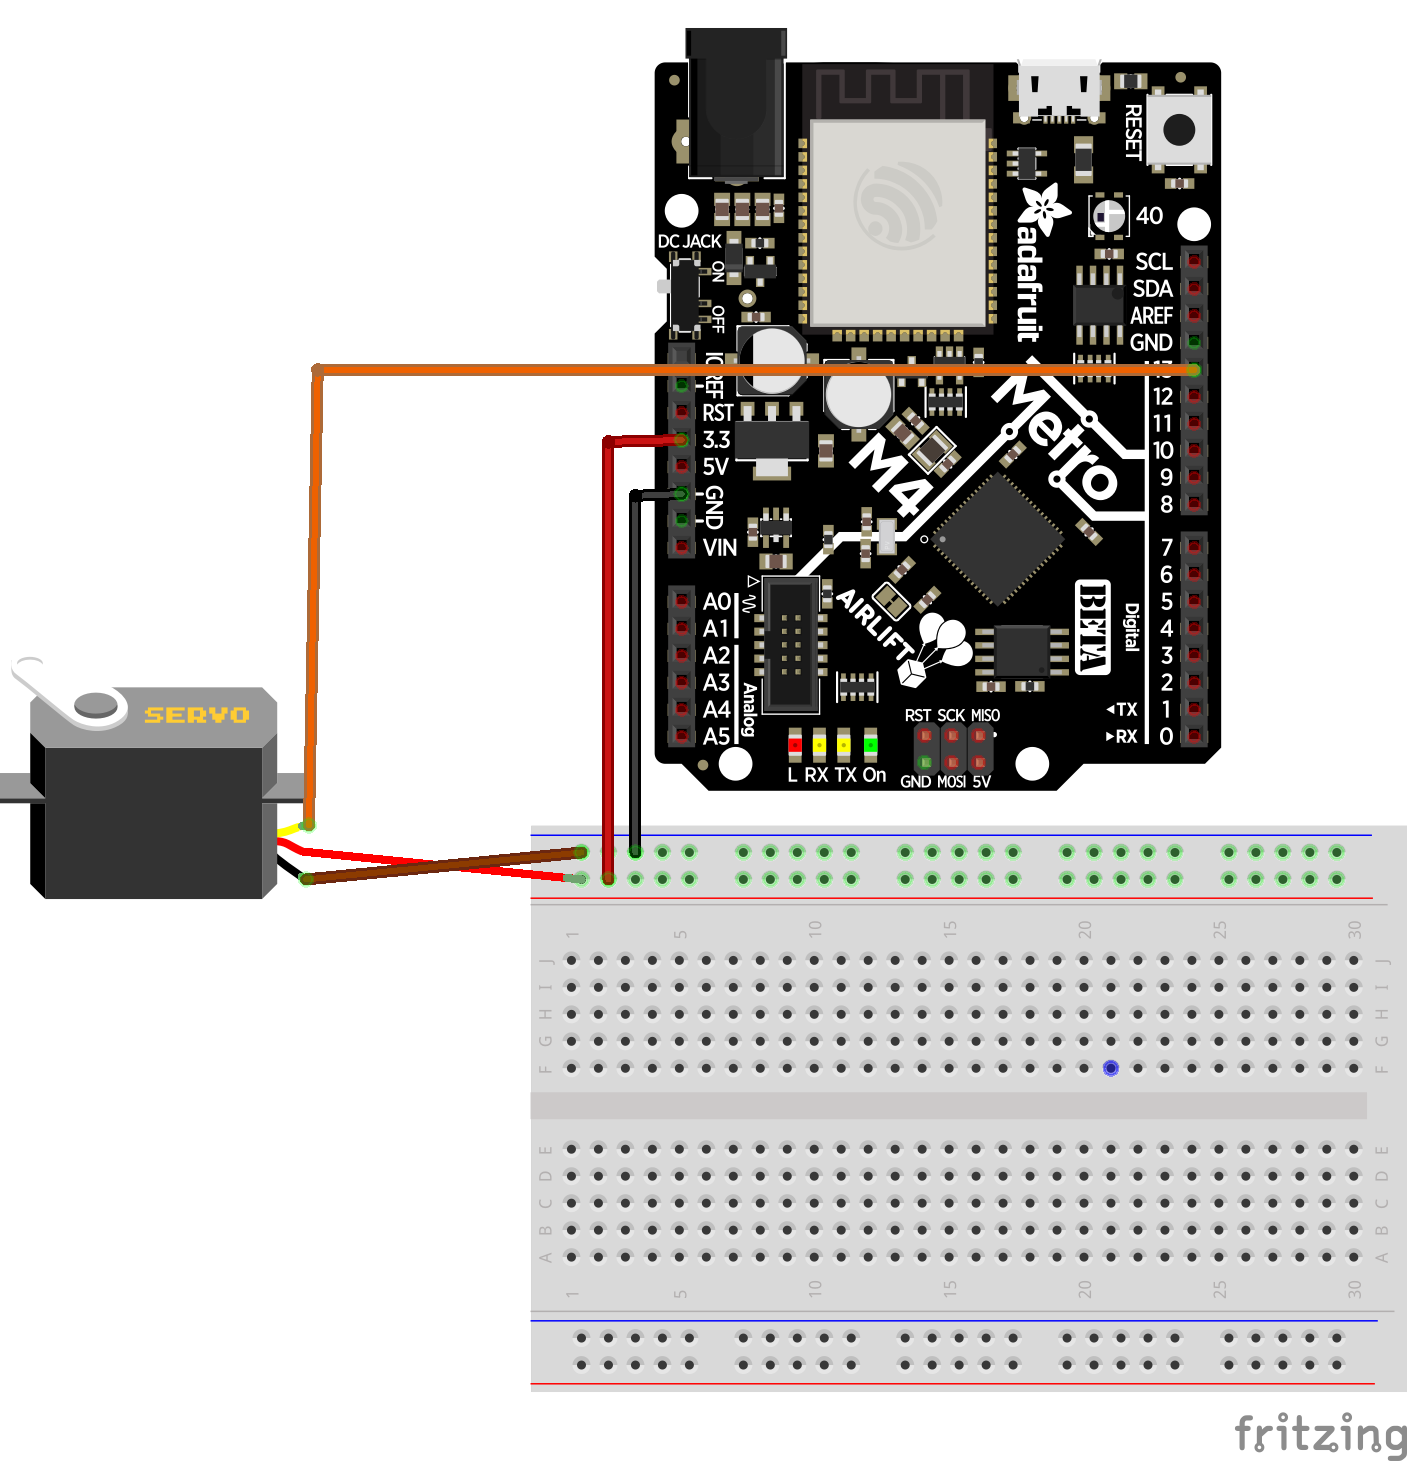
\includegraphics[width=0.6\linewidth]{figures/Servo.png}}
	\caption{Servo Circuit}
	\label{fig:Servo}
\end{figure}

\newpage
\lstinputlisting{code/Servo.py}
\paragraph{Discussie:} Voor het aansturen van een servo hoef je zelf weinig te programmeren, want adafruit heeft hier een speciale bibliotheek voor in hun CircuitPython library bundel. Deze bundel kan je vinden op \url{https://circuitpython.org/libraries}. Zorg dat de adafruit\_motor map in de lib folder op je bordje staat. \\

Importeer de servo module van de adafruit\_motor bibliotheek en ook de time, board en pulsio modules. Een servo object kan eenvoudig gemaakt worden door een pwm object aan de Servo() functie van de servo module te geven. Daarna kan de hoek van de servo ingesteld worden door objectnaam.angle van het servo object aan te passen. In de code gaat de servo van 0 tot 180 graden en terug.\\


\newpage
\section{Twee DC motoren, een servo en een toeter aansturen met een Joystick} \label{sec:DC_Servo_Toeter_Joystick}
\paragraph{Probleem:} Je wilt twee DC motoren tegelijk besturen afhankelijk van hoe ver de joystick naar voren staat. Je wilt tegelijkertijd een servo besturen afhankelijk van hoe ver de joystick naar links en naar rechts staat. Tot slot wil je de toeter aanzetten als je op de joystick drukt.

\paragraph{Benodigdheden:}
\begin{itemize}
	\item 1x 9V batterij
	\item 1x L298N H-Bridge Motor Driver
	\item 2x DC Motor
	\item 1x Servo
	\item 1x \SI{100}{\ohm} weerstand
	\item 1x \SI{8}{\ohm} Speaker
\end{itemize}

\paragraph{Oplossing}:
\begin{figure}[H]
	\center{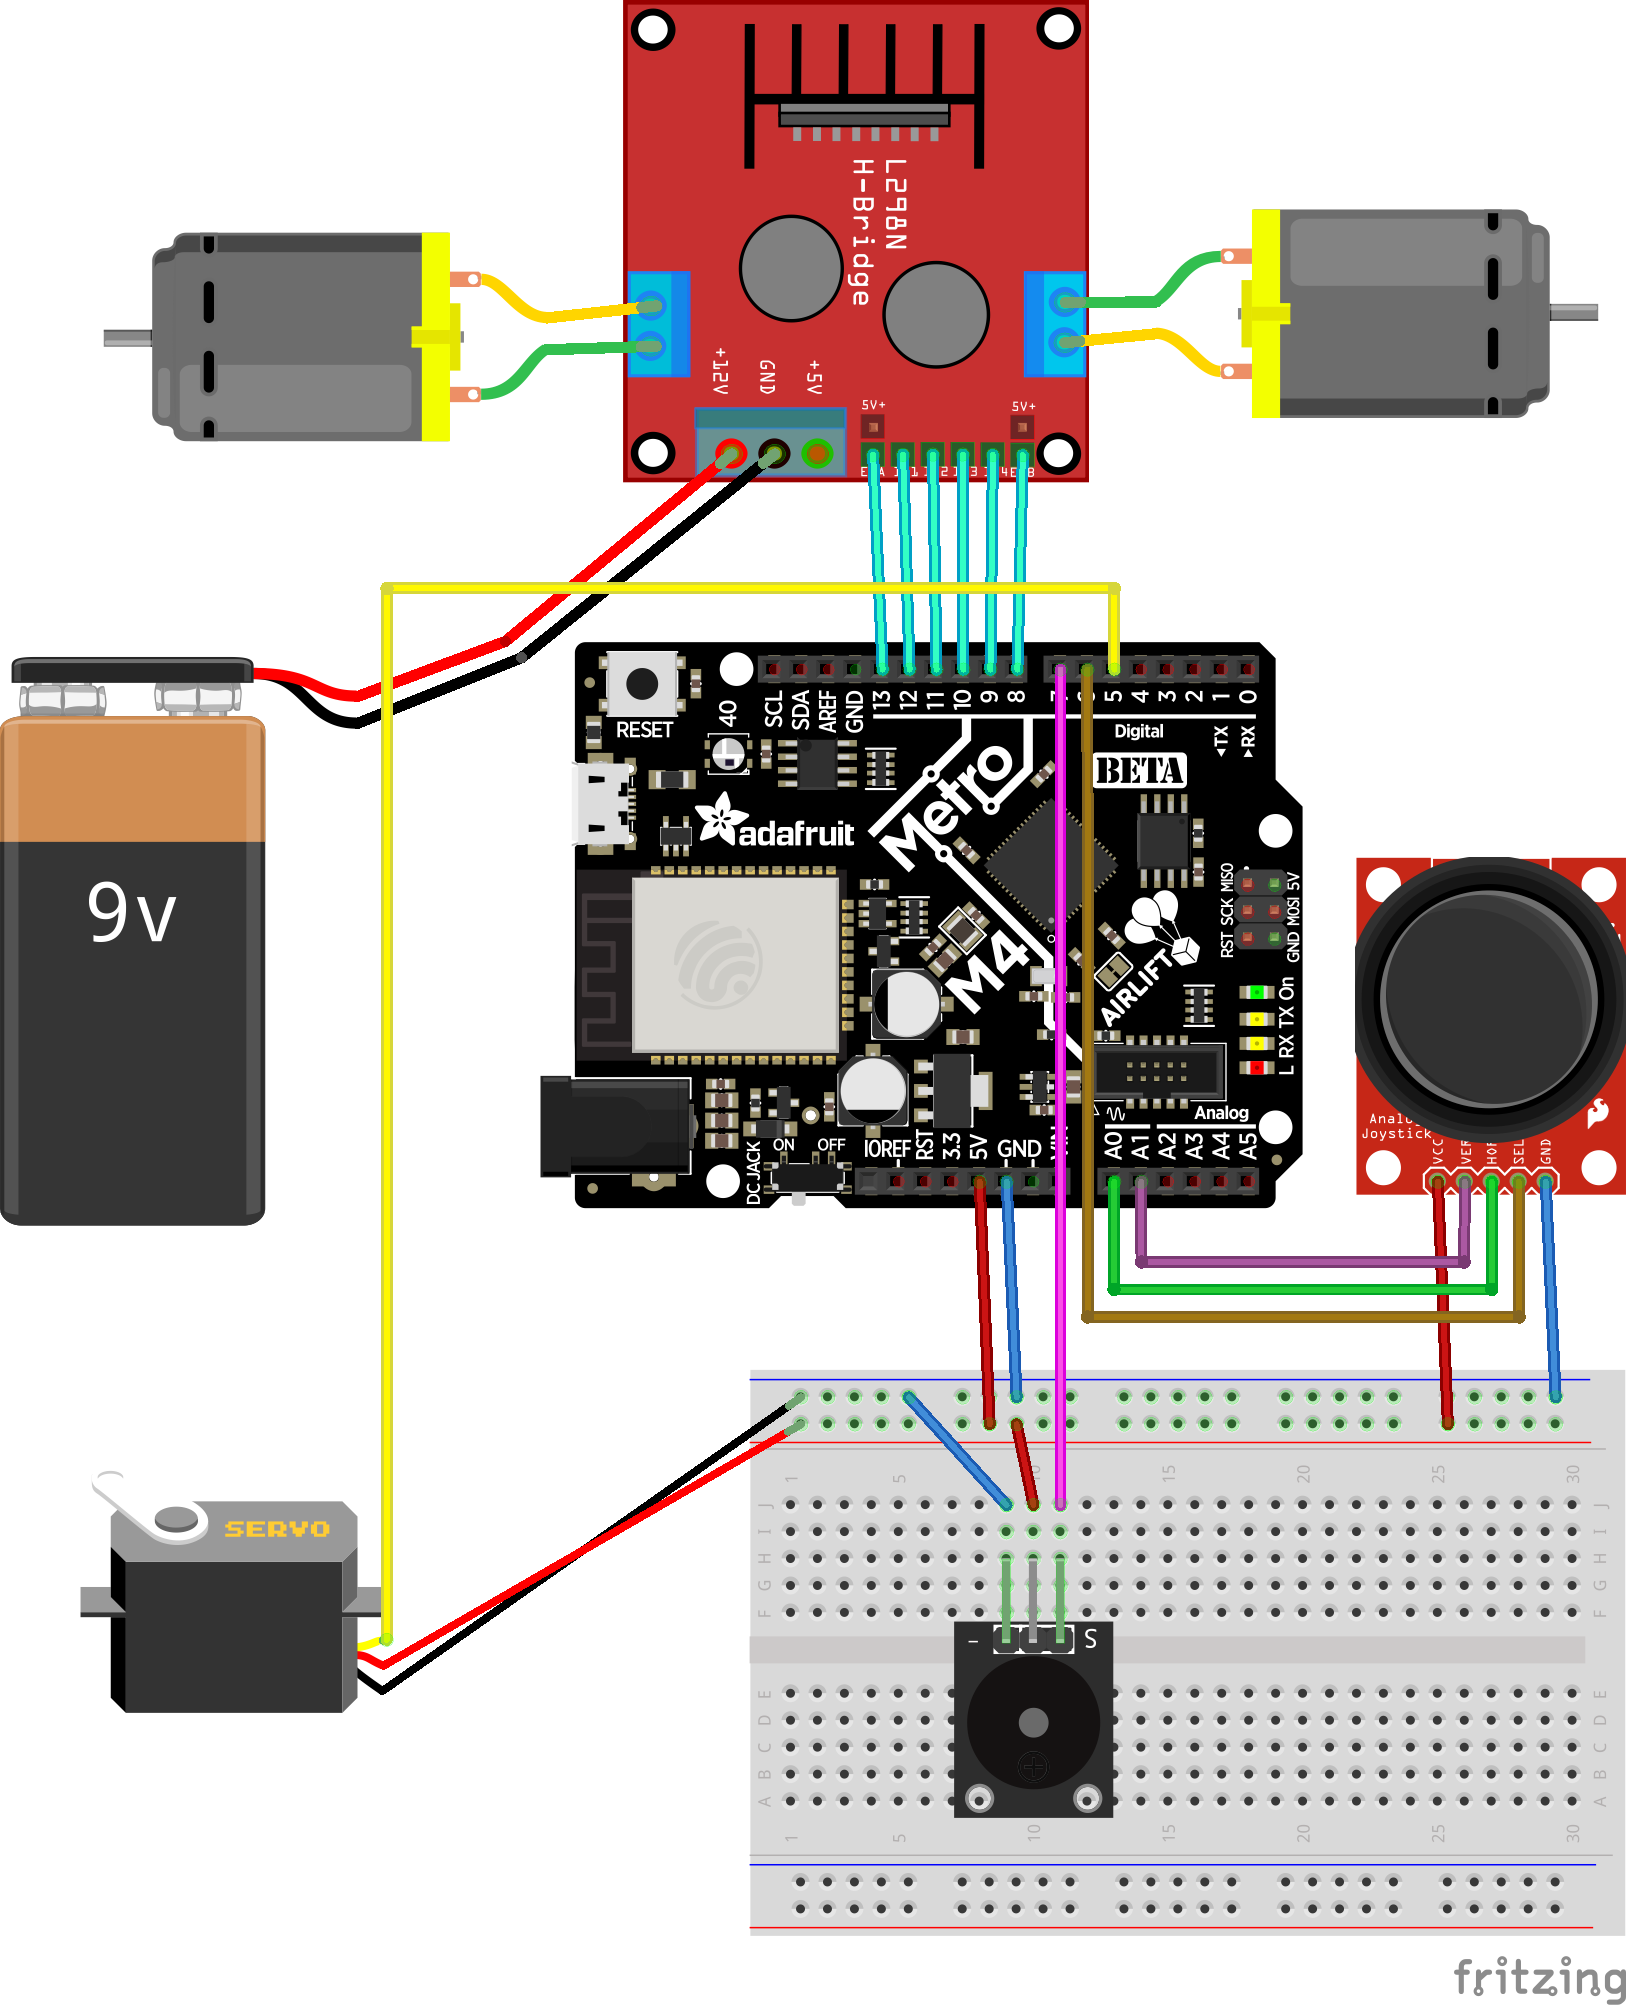
\includegraphics[width=0.7\linewidth]{figures/DC_Servo_Toeter_Joystick.png}}
	\caption{Twee DC motoren, een servo en een toeter aangestuurd door een joystick circuit}
	\label{fig:DC_Servo_Toeter_Joystick}
\end{figure}

\lstinputlisting{code/Two_DC_Motors_Servo_Joystick.py}

\newpage
\paragraph{Discussie:}	Naarmate code meer gaat doen, wordt code vaak ook langer. Het wordt daarom steeds belangrijker om een goede structuur in je code aan te brengen. In deze lap code worden eerst de imports gedaan, daarna de definities, dan de initialisatie en tot slot het programma. 

Vooraf een naam voor de I/O pinnen defini\"eren en later deze naam in de code gebruiken is erg handig. Als je namelijk de ENA pin niet op D13 maar op D2 wilt aansluiten, hoef je alleen de definitie van de ENA\_pin te veranderen en verder niet door de code te zoeken waar je allemaal D13 hebt gebruikt. Ook is het veel makkelijker om te zien of je pinnen per ongeluk dubbel gebruikt.\\

In het kader van het lezen en onderhouden van code kan je zien dat het besturen van een motor in een class is verwerkt. In recept~\ref{sec:TwoDCMotors} moest voor het gebruik van 2 motoren, 2 keer de code voor de initialisatie en voor elke motor een forward() en backward() functie geschreven worden. Als je nog een functie wil schrijven voor het gebruik van de motor, zoals setMotor() in deze code, moet ook dat 2x apart gemaakt worden. Er is een ongeschreven regel in programmeren die zegt 'don't repeat yourself'. Als je jezelf moet herhalen is er vaak een betere manier. 

Het enige verschil tussen de eerste en tweede DC motor is welke pinnen gebruikt worden. De initialisatie en wat er moet gebeuren om de motor voor en achteruit te laten draaien is hetzelfde, alleen moet het dus op andere I/O pinnen gebeuren. Er kan dan een class gemaakt worden voor motoren die de algemene eigenschappen van een motor bij elkaar houdt. Als er een motor is, dan wordt die altijd bestuurd met 3 pinnen. Deze pinnen moeten ge\"initialiseerd worden en worden altijd gebruikt om de snelheid en richting van de motor in te stellen. 

Als dan objectnaam=DC\_Motor() aangeroepen wordt in de code, met als parameters de 3 pinnen, wordt een instantie gemaakt van deze class. Bij het aanmaken van een instantie wordt \textbf{altijd} eerst de \_\_init\_\_ functie doorlopen. Deze initialiseert de pinnen. Elk DC\_Motor object krijgt automatisch zijn eigen forward(), backward() en setMotor() methodes.  Een methode is een functie die hoort bij een class en kan je aanroepen met objectnaam.methode(). De aangemaakte motor1 en motor2 objecten kan je apart aansturen in de code. Je laat motor1 vol vooruit draaien door motor1.forward(1) aan te roepen en motor2 vol achteruit draaien door motor2.backward(1) aan te roepen. Als je een derde motor hebt kan je met 1 regel een extra motor gebruiken.\\

Na de definitie van de class, worden een paar functies gedefinieerd. De "toDutyCycle" functie converteert de uitgelezen 16-bit waarde van de verticale stand van de joystick naar een positieve of negatieve DutyCycle. De "toAngle" functie converteert de horizontale stand naar een hoek en de "setHorn" functie zet de toeter aan als True wordt gegeven als parameter en uit als een False wordt gegeven.\\

Na alle definities worden de motoren, servo, joystick en toeter objecten ge\"initialiseerd. Daarna komt het programma in de oneindige while loop. In deze loop worden de joystick waarden eerst uitgelezen en geconverteerd naar de betekenis van de waarde. JoyStick vol naar achter betekent een duty cycle van -1, vol naar voor +1. Joystick naar links een servo angle van 0 graden, joystick in het midden 90 graden en rechts 180 graden. Knop ingedrukt een waarde True, niet ingedrukt een waarde False. Vervolgens worden deze geconverteerde waarden gebruikt om de motoren, servo en toeter in te stellen.


	\chapter{Netwerken}

\section{Maken van een WIFI access point}\label{sec:AccesPoint}
	\paragraph{Probleem:} Je wilt een privé netwerk creëren door het bordje te gebruiken als WIFI access point.
	
	\paragraph{Oplossing:}
	\lstinputlisting{code/WIFI_AccessPoint.py}
	\paragraph{Discussie:} De Metro M4 Express heeft een tweede processor op het bordje, de ESP32. De ESP32 heeft WIFI en de coprocessor wordt gebruikt om het netwerk en communicatie over het netwerk te regelen. De ESP32 kan niet direct geprogrammeerd worden en het instellen en communiceren met de coprocessor gebeurt via SPI communicatie. De details hiervan zijn onbelangrijk, omdat Adafruit een bibliotheek heeft die deze communicatie regelt. Je hoeft dus alleen te weten hoe je gebruik maakt van deze bibliotheek. Zorg ervoor dat de adafruit\_esp32spi bibliotheek up to date is en in de lib folder staat op je bordje, zie hoofdstuk~\ref{sec:library}.
	
	Als je gebruik wilt maken van de ESP32 zijn altijd dezelfde 5 regels code nodig om controle te krijgen over de ESP32. Deze stappen zijn te zien onder de comment "setup ESP32 control". De laatste stap cre\"eert een esp object met een heleboel mogelijkheden voor het gebruik van het netwerk. \'E\'en daarvan is het opzetten van een access point. De create\_AP() methode heeft als eerste parameter de naam van het netwerk en als tweede parameter het password. "Pass" in de while loop zorgt dat de loop niks doet, maar het programma wel blijft draaien. Als het programma klaar is wordt het netwerk namelijk gelijk weer afgebroken. Als alles goed gegaan is, staat de naam van je gecreëerde netwerk tussen je WIFI netwerken, zoals in Figuur~\ref{fig:AccessPoint}. Als je inlogt op dit netwerk heb je geen toegang meer tot het internet, omdat dit een priv\'e netwerk is.
	
	\begin{figure}[!htb]
		\center{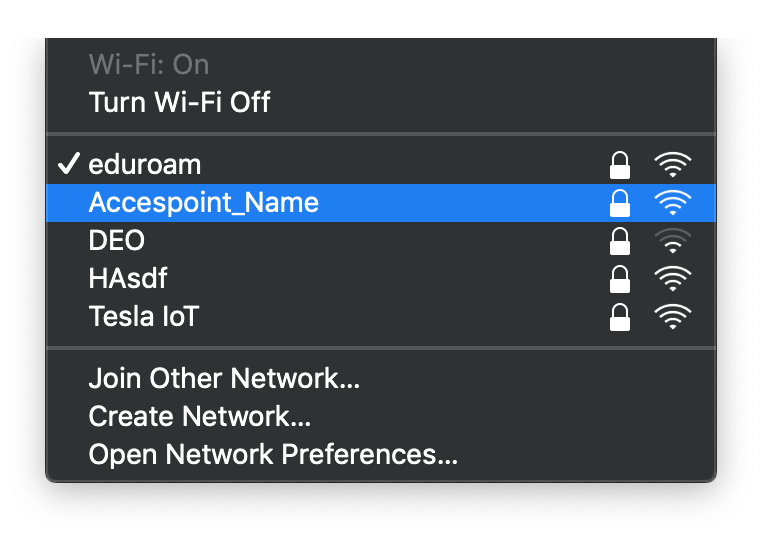
\includegraphics[width=0.6\linewidth]{figures/AccessPoint.png}}
		\caption{Access point in WIFI netwerken}
		\label{fig:AccessPoint}
	\end{figure}
	
	\paragraph{Meer informatie}\textbf{:}\\
	\url{https://circuitpython.readthedocs.io/projects/esp32spi/en/latest/api.html}


\section{Data sturen van client naar server over WIFI}\label{sec:WIFIdata}
	\paragraph{Probleem:} Je wilt over het WIFI netwerk data sturen naar het bordje en dit vervolgens printen naar de terminal.
	
	\subsection{Server}
		\paragraph{Probleem:} Je moet data kunnen ontvangen op je bordje via WIFI.
		\paragraph{Oplossing}: 
		\lstinputlisting{code/Minimal_Server.py}
		\paragraph{Discussie:} De code lijkt op het eerste gezicht heel complex en om het helemaal goed te begrijpen heb je kennis nodig over netwerk communicatie. Dat gaat dit project te buiten. Gelukkig is de code goed te gebruiken zonder al die kennis en is een globaal idee goed genoeg. 
		
		Om data uit te wisselen tussen het bordje en een ander apparaat zijn 2 dingen nodig. Ten eerste moeten de apparaten op hetzelfde netwerk zitten, dit wordt gedaan door met het bordje een priv\'e netwerk te cre\"eren en als access point te functioneren, zoals in ~\ref{sec:AccesPoint}. Ten tweede moet over dit netwerk een verbinding gemaakt worden tussen de twee apparaten, waarover ze informatie kunnen versturen. Let goed op dat er een verschil is tussen een netwerk en een verbinding. Heel het "world wide web"(internet) zit op hetzelfde netwerk, maar je hebt met je computer niet met alle websites een verbinding. 
		
		Achter de schermen draait een website op een \textit{server}. Een server is een computer dat een programma draait dat wacht tot een ander apparaat, een \textit{client}, een verbinding maakt. De client stuurt dan een datapakketje naar de server, waarin naar de gewenste pagina wordt gevraagd. De server ontvangt dit datapkketje, leest de aanvraag en stuurt de gewenste pagina terug naar de client.
		
		Dit principe wordt ook gebruikt voor het communiceren tussen je bordje en je computer. Eerst wordt een in de code een WIFI netwerk gecre\"eerd. Daarna wordt een server gestart op de esp32 met de adafruit\_esp32spi bibliotheek. Deze server wacht tot een client verbinding maakt. Dan gaat de code naar de oneindige while loop die uit 2 stukken bestaat. Het 1e stuk bevat nog een while loop, waar de code blijft loopen tot een client verbinding maakt. Als er dan een verbinding is gaat het door naar het 2e stuk met de if/elif statement. Er wordt gekeken of er een verbinding is en of er data is gestuurd door de client. Als dat het geval is wordt de data gedecodeerd en geprint naar de terminal. De plaats waar de print statement staat is de plek waar je ook andere dingen kan doen met de data, zoals motors aansturen en data terugsturen(zie recept~\ref{sec:RCservo}). Zolang de verbinding bestaat worden het eerste stuk met de while loop en het stuk met de elif statement overgeslagen en wordt alleen de if statement uitgevoerd als er data is verstuurd door de client. Anders gebeurt er niks en blijft het loopen tot er wel iets is gestuurd of de verbinding wordt verbroken. Als de client de verbinding verbreekt wordt de elif statement uitgevoerd en komt de code terug in de while loop, waar het programma wacht op een nieuwe verbinding.


\newpage
\subsection{Client}
	\paragraph{Probleem:} Je wilt data sturen naar een server vanaf je pc.
	\paragraph{Oplossing:}
	\lstinputlisting{code/Minimal_Client.py}
	\paragraph{Discussie:} De \textbf{client} kant moet niet ge\"upload worden op je bordje, maar moet je runnen met python op je computer. Houd er rekening mee dat de code alleen werkt als je op hetzelfde netwerk zit als je bordje. Log dus eerst in op het WIFI netwerk van je bordje.
	
	Verbinding maken met- en data sturen naar een server kan eenvoudig met de socket module van Python's standaard bibliotheek. Je geeft de server's host adres en port nummer en met 3 regels code kan je verbinden met de server. 
	
	In de oneidige while loop wordt de gebruiker gevraagd om een bericht te typen. Als dit bericht '-q' is wordt het programma afgesloten en anders wordt het geconverteerd naar een bytearray dat kan worden verstuurd met de sendall() methode van de socket library. Als het goed is zie je de text die je stuurt verschijnen in de REPL van Mu editor.
	


\section{Besturen van een servo met laptop}\label{sec:RCservo}
\paragraph{Probleem:} Je wilt over WIFI een servo aansturen.
\newpage
\subsection{Server}
\lstinputlisting{code/RC_Servo.py}

\subsection{Client}
\lstinputlisting{code/RC_Servo_Client.py}

\paragraph{Discussie:} Dit is een combinatie van het sturen van data over WIFI in recept~\ref{sec:WIFIdata} en het aansturen van een servo in recept~\ref{sec:servo}. Het enige verschil aan de \textit{Client} kant ten opzichte van recept~\ref{sec:WIFIdata} is dat je een hoek moet invoeren. Aan de server kant is het verschil dat de servo geinitialiseerd wordt en dat in plaats van data te printen, nu de hoek van de servo ingesteld wordt. 

\section{Gebruiken van keyboard toetsaanslagen}
\paragraph{Probleem:} Je wilt in een programma het keyboard van je laptop gebruiken.
\paragraph{Oplossing:}
\lstinputlisting{code/PrintKeyStroke.py}
\paragraph{Discussie:} Voor het gebruik van je keyboard heb je de python bibliotheek "keyboard" nodig. Open de terminal op je laptop en type: \newline
\\
pip install keyboard\\
\\
In de code wordt eerst de bibliotheek keyboard ge\"importeerd. Daarna wordt de functie gedefinieerd die bepaald wat er gebeurd als je een toets indrukt. Met keyboard.hook(functienaam) koppel je het keyboard aan de functie en 'luistert' het programma op de achtergrond naar toetsaanslagen. Bij een keyboard event, zoals het indrukken of loslaten van een toets, wordt de lopende code onderbroken en wordt een eventobject doorgegeven aan de functie. Het eventobject heeft de eigenschappen "name" en "event\_type". De name eigenschap is de toets en event\_type zegt of de toets is ingedrukt of losgelaten. In de oneindige while loop hoeft verder niks geprogrammeerd te worden, omdat door keyboard.hook() op de achtergrond geluisterd wordt. Het zou kunnen dat je de code als administrator moet runnen. Als de code werkt, worden de toetsnaam en toetsrichting naar de terminal geprint.
\\
\url{https://pypi.org/project/keyboard/}

\newpage
\section{Gebruik van keyboard om een Servo aan te sturen over WIFI}
\paragraph{Probleem:} Je wilt over WIFI met je keyboard een servo aansturen.

\paragraph{Benodigdheden:}
\begin{itemize}
	\item 1x Servo
\end{itemize}

\begin{figure}[H]
	\center{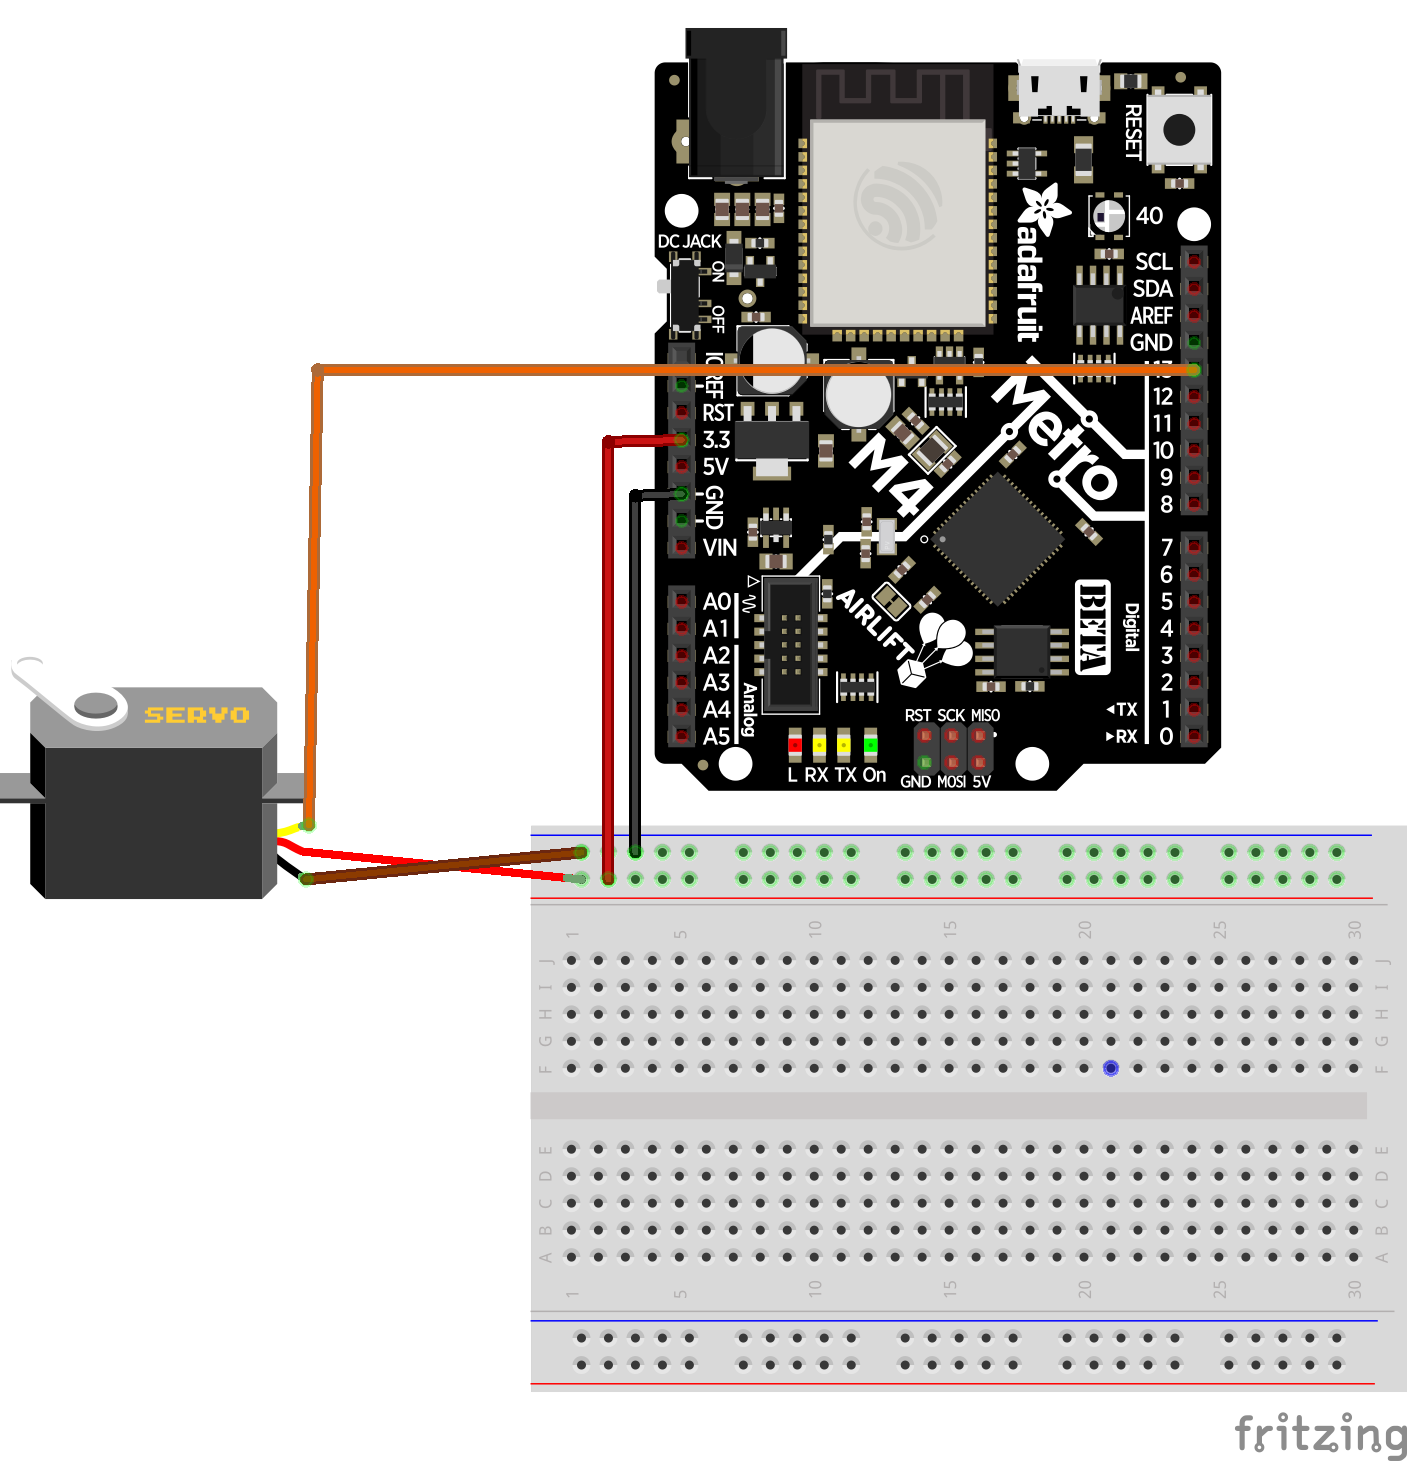
\includegraphics[width=0.6\linewidth]{figures/Servo.png}}
	\caption{Servo Circuit}
	\label{fig:ServoKeyboard}
\end{figure}


\subsection{Client:}\label{sub:KeyboardServoClient}
\paragraph{Oplossing:}
\lstinputlisting{code/Keyboard_Servo_Client_v2.py}


\paragraph{Discussie:} Om een servo met een keyboard te besturen over WIFI moeten 2 dingen gebeuren. Ten eerste moet bijgehouden worden welke knoppen zijn ingedrukt en ten tweede moet deze informatie over het netwerk gestuurd worden.\\\\

Laten we eerst kijken naar het bijhouden van welke knoppen zijn ingedrukt. Een dictionary met de naam button\_state wordt ge\"initialiseerd met de keys 'left' en 'right' om dit bij te houden. Om te zien hoe de dictionary gebruikt wordt, moeten je kijken naar de 3 functies om key events te regelen. De key\_handler() functie is de functie die met keyboard.hook() gebonden wordt aan het keyboard. Bij elk keyboard event wordt het programma onderbroken en wordt key\_handler() gerund. De key\_handler() functie kijkt dan of een knop is ingedrukt of losgelaten en stuurt het key\_event dan door naar de key\_press\_handler() functie als een knop is ingedrukt en naar de key\_release\_handler() als een knop is losgelaten. Deze functies kijken vervolgens om welke knop het gaat en zet in de button\_state dictionary een 1 als de knop is ingedrukt en een 0 als een knop is losgelaten. \\

Om deze informatie te sturen over het netwerk moet eerst een netwerk connectie gemaakt worden. Het maken van een netwerk en het sturen van data is al besproken in ~\ref{sec:WIFIdata} en ~\ref{sec:RCservo}. De data moet nog wel in een goede vorm gezet worden, zodat het over het netwerk gestuurd kan worden. Dit wordt gedaan in de infinite while loop. Eerst wordt de knoprichting bepaald van button\_state. Als alleen rechts is ingedrukt krijgt keyDirection de waarde 1, als alleen links is ingedrukt -1, als rechts en links zijn ingedrukt 0 en als niks is ingedrukt ook 0. \\

Voordat keyDirection over het netwerk gestuurd wordt, wordt gekeken of de richting anders is dan de laatst gestuurde waarde. Alleen als de waarde is veranderd wordt de nieuwe waarde over het netwerk gestuurd. Dit wordt gedaan om het netwerk te ontlasten. Het controleren van de verandering is de taak van de checkStateChange() functie, waar keyDirection vergeleken wordt met current\_direction en een 0 of 1 terug geeft als de richting respectievelijk niet of wel is veranderd. Als de richting is veranderd gaat het programma de if statement in. Eerst wordt de waarde met de sendData() functie gestuurd. In deze functie wordt keyDirection eerst verandert in een alfabetische letter met het gebruik van de PACK\_DICT. De waarden op deze manier "coderen" maakt het een stuk eenvoudiger om de data na het sturen weer uit te pakken. 
Data wordt namelijk byte voor byte verzonden. \'E\'en string character is gelijk aan 1 byte. Als je de waarde -1 converteert naar de string '-1' moeten 2 bytes verstuurd worden, de - en de 1. Deze variabele lengte maakt waarden uitpakken aan de kant van de ontvanger een stuk complexer, mede doordat meerdere waarden in de buffer kunnen staan. De waarden 0,1,0,-1,0,-1 uit de string "010-10-1" vereist meer dan alleen splitsen, omdat er soms 1 en soms 2 characters gebruikt worden voor een waarde. "bcbaba" splitsen in b,c,b,a,b,a en vervolgens omzetten met een dictionary in 0,1,0,-1,0,-1 maakt dit heel eenvoudig. 
Na het coderen van de waarden in de sendData() functie, wordt de character met .encode() verandert in binaire data en vervolgens verstuurd met sendall().
Tot slot wordt current\_direction ge\"updatet en wacht het programma \SI{50}{\milli\second} voordat het opnieuw de while loop doorloopt. 


\newpage
\subsection{Server}\label{sub:KeyboardServoServer}
\paragraph{Oplossing:}
\lstinputlisting{code/Keyboard_Servo_Server_v2.py}


\paragraph{Discussie:} De server kant is voor het grootste deel te vergelijken met \ref{sec:RCservo}. Het grootste verschil is wat voor data er binnen komt en hoe hier mee omgegaan wordt. De data wordt uitgelezen in de oneindige while loop met de recv() methode. We verwachten hier van de client kant een gecodeerde character of een string met characters, afhankelijk van hoeveel er gestuurd zijn en in de buffer staan. We zijn alleen ge\"interesseerd in de laatste character, omdat deze de recentste toestand weergeeft en moeten deze destilleren van de buffer. De bytearray wordt eerst geconverteerd naar een string en vervolgens wordt de laatste character uit de string gehaald. Deze alfabetische letter wordt gedecodeerd met de UNPACK\_DICT. UNPACK\_DICT is een soort van de omgekeerde PACK\_DICT, alleen wordt a,b,c nu omgezet in de servo waarden 0, 90, 180, in plaats van de toetswaarden -1,0,1. Na het destilleren van de laatst gestuurde waarde kan gelijk de servo ingesteld worden.\\



	\chapter{Remote Controlled boot}
Alle delen om een RC boot te maken zijn nu behandeld, wat in dit hoofdstuk gebeurd. De client kant is een uitgebreide versie van ~\ref{sub:KeyboardServoClient} en de Server of boot kant is een combinatie van ~\ref{sec:DC_Servo_Toeter_Joystick} en ~\ref{sub:KeyboardServoServer}.


\section{Circuit}
\begin{figure}[H]
	\center{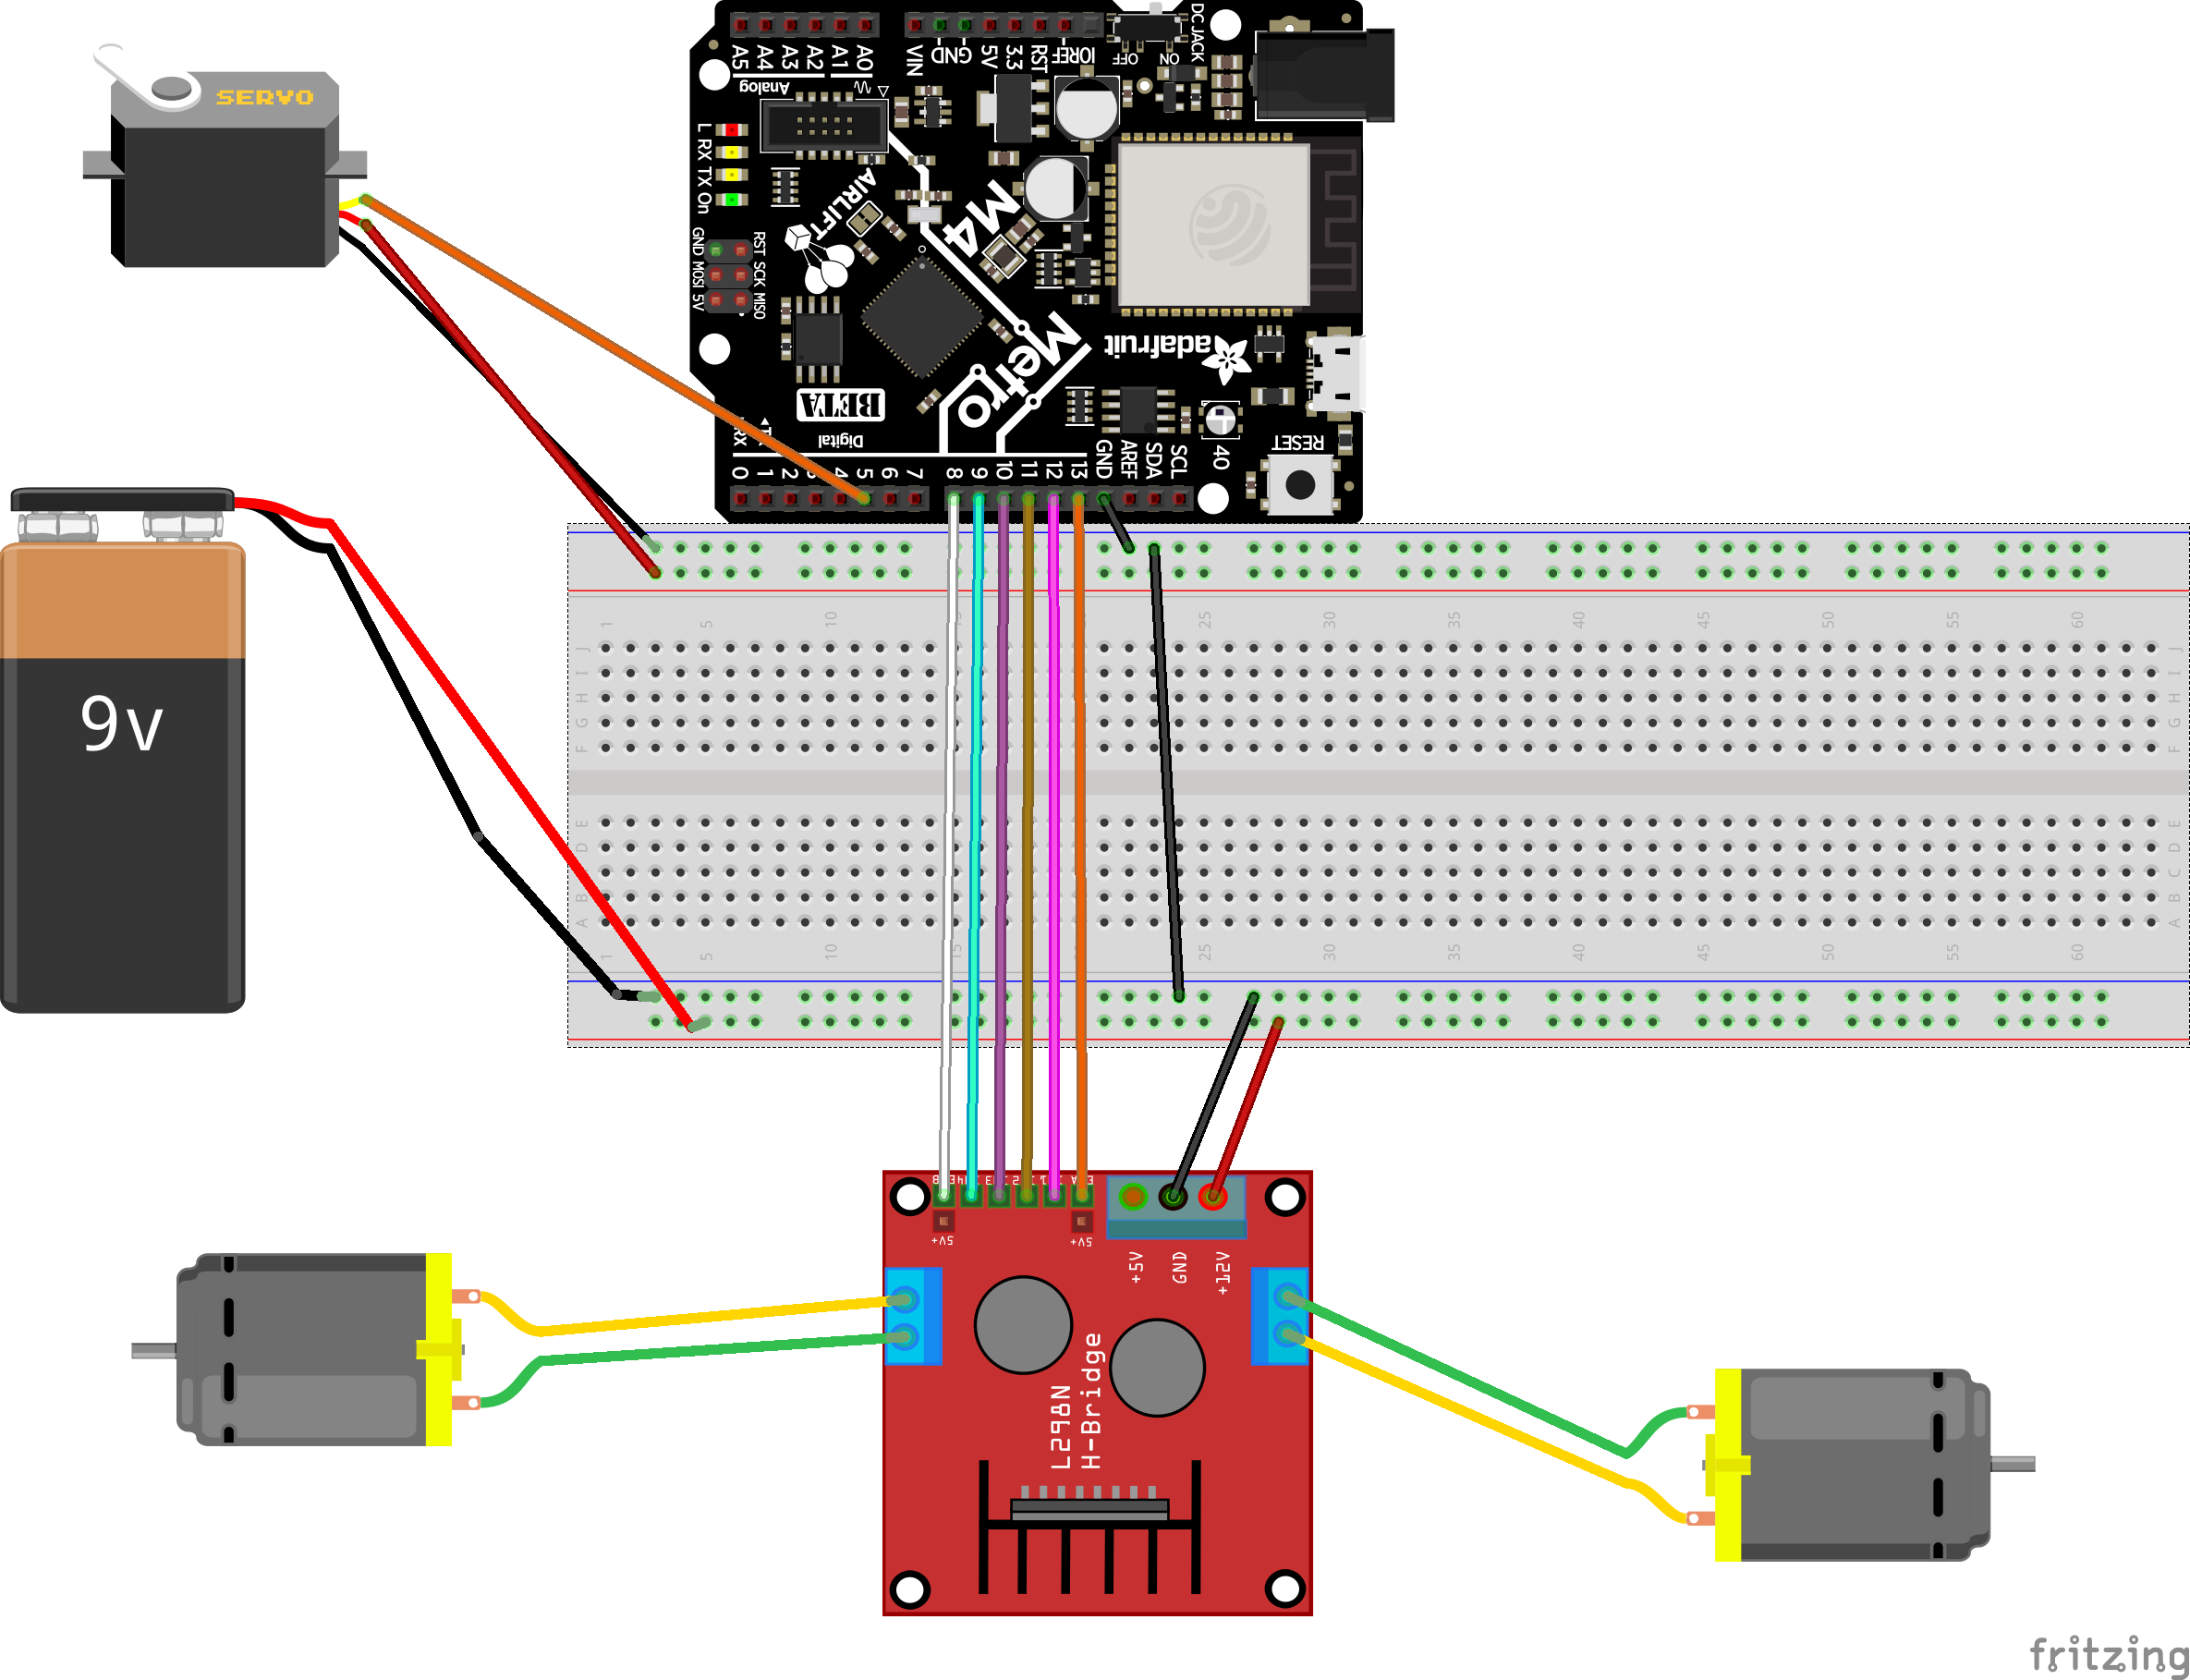
\includegraphics[width=0.8\linewidth]{figures/RC_Boat.png}}
	\caption{Circuit voor het aansturen van een boot}
	\label{fig:RCBoat}
\end{figure}

\newpage

\paragraph{Benodigdheden:}
\begin{itemize}
	\item 1x Servo
	\item 2x DC motor
	\item External power source
	\item 1x L298N H-Bridge Motor Driver
\end{itemize}

\section{Code}
\subsection{Computer client side}
\paragraph{Oplossing:}
\lstinputlisting{code/RCBoat_Client_v2.py}
\paragraph{Discussie:} De code is eigenlijk precies hetzelfde als recept~\ref{sub:KeyboardServoClient}. Er is weer de key\_handler() functie die wordt aangeroepen bij een keyboard event. De functie stuurt het event door naar de key\_press\_handler() als een toets is ingedrukt en naar de key\_release\_handler als een toets is losgelaten. Er is de functie sendData() voor het coderen en sturen van data en een functie checkStateChange() om te controleren of er een verandering is ten opzichte van de laatst gestuurde richting. Het enige verschil is dat de PACK\_DICT, button\_state en functies uitgebreid zijn met de "up" en "down" toetsen. Als de code niet duidelijk is lees dan recept~\ref{sub:KeyboardServoClient} nog een keer.

\newpage
\subsection{Boat server side}
\paragraph{Oplossing:}
\lstinputlisting{code/RCBoat_Server_v2.py}
\paragraph{Discussie:} Deze code is een combinatie van recept~\ref{sec:DC_Servo_Toeter_Joystick} en recept~\ref{sub:KeyboardServoServer}. Eerst worden imports en definities gedaan. Daarna wordt de DC\_motor() class gedefinieerd die is hergebruikt van recept~\ref{sec:DC_Servo_Toeter_Joystick}. 
Na de definities worden de servo, dc motoren en het netwerk ge\"initialiseerd en gaat het programma de oneindige while loop in. Zodra het een connectie heeft leest het de gestuurde data uit, converteert de data naar een string, haalt de laatst gestuurde character uit de string en zoekt de bijbehorende tuple op in de dictionary. Vervolgens wordt de tuple en uitgepakt in een rudderAngle en een motorvalue die tot slot worden gebruikt om de servo en motoren in te stellen. 








	
	%\input{Conclusion}
	
	\appendix
	
	
	
\end{document}          
